\chapter{Case Study 1: Population Health Impacts Of Climate Heating}
\openepigraph{%
	A ruined planet cannot sustain human lives in good health. A healthy planet and healthy people are two sides of the same coin.
}{Dr. Margaret Chan, Executive Director, WHO}

\marginnote{
	\newthought{Key Message:} The impact of climate heating on local populations is a truly wicked problem that public health practitioners spend very little time thinking about. It's too hard. It isn't a health system priority; it is tomorrow's problem. We need to make it easier to understand and incorporate into all local population planning. Systems thinking might provides some useful tools.
}

\section{Complexity and Public Engagement}
The aim of this document is to bring together all threads of this project that set out to explore how public health could develop policy in the area of potential health impacts from climate change on the older population of West Dorset. It became obvious quite early in the project that this was not going to be an easy task. The difficulty arises firstly in developing a meaningful engagement on the topic. Getting attention for a problem that is in the future, and not thought to be more significant in impact than many current population health issues was always going to be a challenge.

We have approached this challenge by adopting a `systems thinking' approach to our engagement with policy makers and `futures studies' approach in our engagement with the community more widely. In truth, these approaches are complementary and underpin both engagement processes.

\begin{description}
	\item[Systems Thinking]An approach to developing deeper understanding of complexity by examining problems and challenges within the context of the `system' in which they exist.
	\item[Futures Studies] An approach to the development of strategy that seeks to understand an issue or challenge in the context of a more comprehensive picture of a future state. Incorporates a fundamental belief that at any point in time there are many possible futures -- strategically one should work towards a preferred future.
\end{description}

\subsection{Change of Project Emphasis}
The project that began as a climate change impacts on the health of older persons in West Dorset, ended as a project entitled, \emph{Complex Challenges \& Public Engagement}, reflecting the broader issues we encountered during the running of this project.

Our change in emphasis was not an abandonment of the initial research focus that sought to develop a better understanding of what impacts older people in West Dorset would face in thirty years. Indeed, it was our desire to make a meaningful contribution in this area that we realised that our initially more traditional research approach had two shortcomings:
\begin{enumerate}
	\item Scientific uncertainties regarding the estimated outcomes 30 years in the future are such that we would not succeed in delivering new information, but rather our approach would include the same lists of possible outcomes and generalised mortality outcomes; and
	\item Consequently, the initial difficulties we experienced in engaging stakeholders would be compounded, because we had nothing particularly compelling to engage with.
\end{enumerate}

\subsection{Project Outputs}
Thus far this project has presented a number of workshops, a conference poster and delivered a systems model and story, various futuring deliverables including a Futures Story and this report.

It is anticipated that these materials will be used further in 2016 to continue exploring the public health challenge faced by climate change in Dorset and we will also seek to publish some of this work.

Furthermore, a longer term outcome will require a longer effort as we attempt to apply the methods explored here to other public health challenges over the coming years.

\subsection{Project Outcomes}

Ultimately, Public Health Dorset role is to protect and improve the health of its population -- we hope that methods adopted during this project will contribute towards the success of that role. However, a more immediate outcome has been the exposure of many staff to systems thinking and futuring methods, which now extends their potential reach in developing shared understanding of particularly complex public health challenges.

\subsection{Report Organisation}

Part I of this report focusses on the `systems thinking', `systems modelling' and `systems story telling' methods that were used in an effort to develop a shared understanding of this public health challenge.

Part II reports on the use of future methods: `horizon scanning', `scenario building' and `futures story telling'.

Part III of this report serves as a repository for presentations and stakeholders events, recording the evolution of the group's thinking over the two year life of the project.

\subsection{Public Health and Systems Thinking}
Systems Thinking as an approach to problem solving appears to have evolved from a sub-discipline of Engineering, Systems Dynamics, and the work of Jay Forrester.\cite{WikipediaJWF} However, it has been used more broadly to explore problems in natural systems, business and organised problem solving more generally.\cite{Ford2010, Senge2006, MaaniCavana2007}

The articulation of systems thinking as a tool in the practice of public health has only occurred relatively recently in explicit reference to `systems', ``The whole concept of public health is founded on the insight that health and illness have causes or conditions that go beyond the biology and behaviour of the individual human being''.\cite{Midgley2006} While, this has always been implicitly understood in modern public health, 

\begin{quotation}
\ldots there is no single operational method for identifying and interpreting these relationships, there is, in fact, a common conceptual orientation recognizable as a systems approach: it is a paradigm or perspective that considers connections among different components, plans for the implications of their interaction, and requires transdisciplinary thinking as well as active engagement of those who have a stake in the outcome to govern the course of change.\cite{Leischow2006}
\end{quotation}

It is clear that a systems approach is intuitively sensible and that the methods available have matured to make its adoption in public health practice both timely and practicable.\cite{Trochim2006, Homer2006} Nonetheless, we still to this day have relatively few examples of its use at the `coal face', and the authors of these works are academics and management consultants.

More recent work looking at the use of a systems approach in disentangling health disparities and health system policy are aimed at experts in their respective fields and not at developing a shared understanding of the public health challenge to public health practitioners.\cite{Roux2011} Indeed, one could question the degree to which these authors truly understand sytems thinking and the application of causal loop and other methods when talking of `health systems' and making only the most rudimentary attempt to actually visualise and map the system.\cite{BoschCapblanch2012} Nonetheless, the effort to improve the targeting of these methods and make a difference in public health continues,

\begin{quotation}
Recognizing that a problem exists and taking action to solve a problem are two activities that many do well, but there is an in-between step that often receives inadequate attention. The source of all important management blunders can be traced back to a mistake in accurately discerning what is important in a situation and incorrectly formulating a problem to be addressed.\cite{Canyon2013}
\end{quotation}

\section{Health Impacts of Climate Change on an Ageing Population}

With this background of a rather recent and not-so-successful introduction of public heath to systems thinking methods, we have focussed on a systems approach because it seemed the only way to adequately address this problem in a way that would make meaningful communication with all stakeholders possible.

\subsection{The Big Picture}
There is a scientific consensus that anthropogenic climate change is increasing global temperature and that this will continue for at least another century. This will impact human health and well-being because the links to human health and climate are well understood.

\begin{quotation}
The health of human populations is sensitive to shifts in weather patterns and other aspects of climate change (very high
confidence). These effects occur directly, due to changes in temperature and precipitation and occurrence of heat waves, floods, droughts, and fires\ldots Until mid-century climate change will act mainly by exacerbating health problems that already exist (very high confidence)\ldots (p. 713)\cite{IPCC2014}
\end{quotation}

The impact of climate change on older persons will be particularly problematic, because

\begin{quotation}
Older people are also more likely to suffer from health conditions that limit the body's ability to respond to stressors such as heat and air pollution\ldots (p. 718)\sidenote{Citation as above.}
\end{quotation}

The range of potential health impacts identified is lengthy and includes:\cite{Portier2010}
\begin{itemize}
\item Asthma, Respiratory Allergies, and Airway Diseases
\item Cancer
\item Cardiovascular Disease and Stroke
\item Foodborne Diseases and Nutrition
\item Heat-Related Morbidity and Mortality
\item Human Developmental Effects
\item Mental Health and Stress-Related Disorders
\item Neurological Diseases and Disorders
\item Vectorborne and Zoonotic Diseases
\item Waterborne Diseases
\item Weather-Related Morbidity and Mortality
\end{itemize}

There have been numerous substantial reviews on the potential health impacts of climate change on the human population and potential mitigation strategies from the WHO\cite{WHO2014a,WHO2014b, WHO2015}, the IPCC\cite{IPCC2014}, the US\cite{Portier2010, Luber2014} and the UK\cite{HPA2012, LancetCom2015}.


The general consensus is that climate change will impact human health in a myriad of ways in the not distant future and that the focus should now turn to mitigation of health impact. There does not, however, appear to be a simple recipe that can be applied and the consequences for much of the developing world will be far more severe than that in the developed world. Nonetheless, scientific evidence suggests that the impacts will be severe and measurable.


\subsection{Temperature Stress Attributable Excess Mortality}
Temperature stress to human physiology, both cold and warm, is relative to whatever is considered to be a 'normal' temperature range. It is important to emphasise that excess mortality related to cold and warm temperature stress is evident at very average temperatures. A recent English study indicates that local temperature stresses occur over very average temperature ranges.\cite{Hajat2014}

In Dorset, UK, temperature stress is estimated to occur when it is either warmer than 17.6 deg C or cooler than 12.1 deg C. The relative risk (RR) of death increases by approximately 2\% for each degree C beyond these thresholds (Figure~\ref{fig:rr}).

As a consequence of Dorset's ageing population, excess winter mortality in the Southwest will continue to be far more of a problem than excess heat related deaths even in a warmer world of 2044. This counter-intuitive finding is entirely driven by the demographic trend of an ageing population.


\begin{figure}[htbp]
\centering
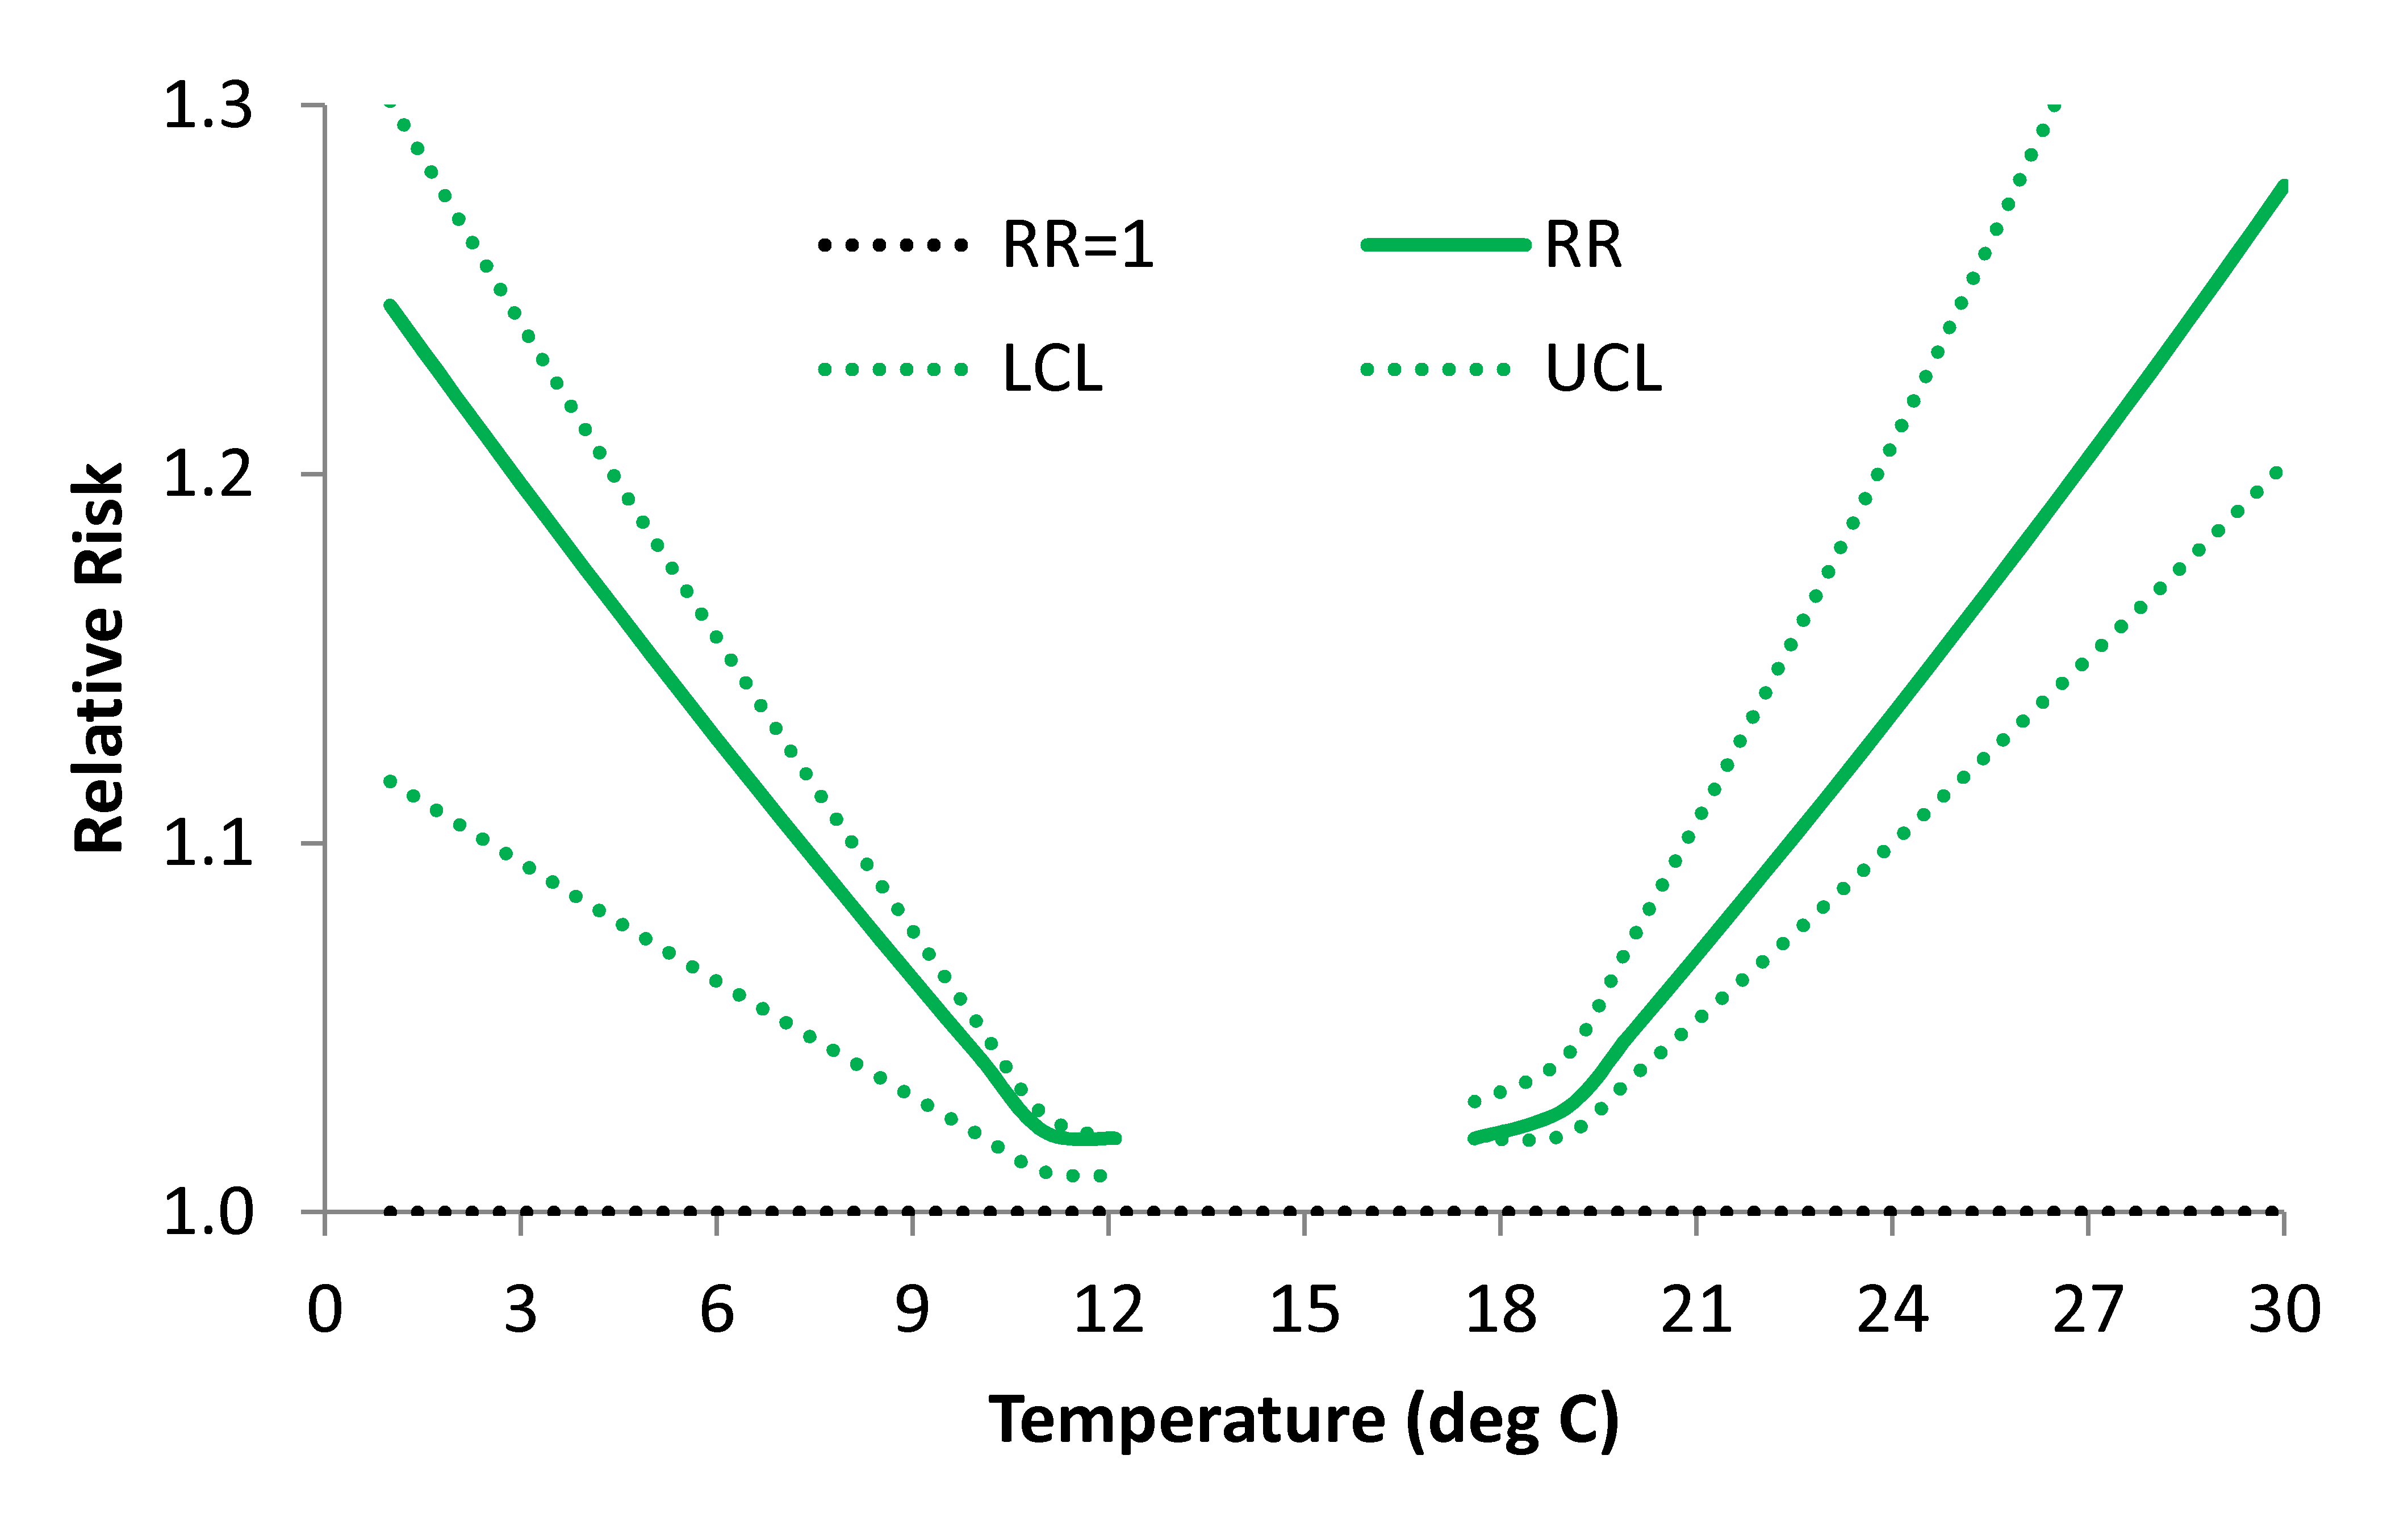
\includegraphics{CCA/img/RRgraph.png}
\caption[Relative Risk and Temperature]{The relative risk (RR) of death increases by approximately 2\% for each degree C beyond these thresholds.\label{fig:rr}}
\end{figure}





%\section{Climate Change}
\subsection{Climate Change Projections for UK}
This simulation model is based upon \href{http://ukclimateprojections.metoffice.gov.uk/media.jsp?mediaid=87867 \&filetype=pdf}{UKCP09 SRES A1B Emission Scenario Projection}, which "provides a basis for studies of impacts and vulnerability and decisions on adaptation to climate change in the UK over the 21st century."\cite{Jenkinsetal2009}

The emission 'story line' that underpins the future climate scenario used in this work is the IPCC's  \href{http://www.grida.no/publications/other/ipcc_sr/?src=/climate/ipcc/emission/}{Special Report Emissions Scenarios}.\cite{IPCC2000}

The Weather Generator is used here to provide a time series of mean daily temperature. It allows users to generate plausible daily time series at 5 km resolution level. As there is no climate change data available at the 5km scale, the Weather Generator 'downscales' the climate data from the 25km scale (Figure~\ref{fig:wgd}).\cite{Jonesetal2010}

\begin{figure}[htbp]
\centering
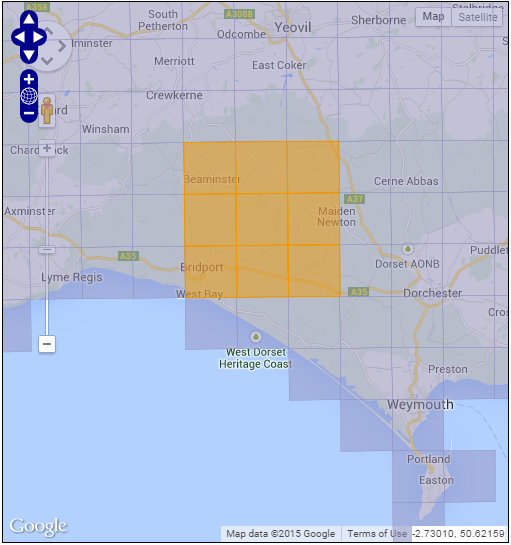
\includegraphics{CCA/img/WGD_WD.png}
\caption{Weather Generator spatial resolution over the West Dorset region.\label{fig:wgd}}
\end{figure}




%\section{Ageing Population}

\subsection{West Dorset Situation Population}
Dorset's population is ageing and this will have be a factor in how severely population health will be impacts by changing climate over the next 30 years. Population ageing, meaning that there will be a greater proportion of the population that is older in the future than is currently the case, is a global trend across the developed western world including the UK. There is a high degree of certainty that this trend will continue well beyond the 30 year reach of this study.

2012-based \href{www.ons.gov.uk/ons/rel/snpp/sub-national-population-projections/2012-based-projections/index.html}{Sub-national Population Projections} for Local Authorities in England, by sex and 5 year age groups, all local authorities and higher administrative areas within England Long-term sub-national population projections are an indication of the future trends in population by age and sex over the next 25 years.\cite{ons2012} They are trend-based projections, which means assumptions for future levels of births, deaths and migration are based on observed levels mainly over the previous five years. They show what the population will be if recent trends continue.

There are a number of uncertainties in ageing and the future of ageing in 2044 that we need to think carefully about:
\begin{itemize}
\item Quality of life, including increased fitness levels
\item Future work/retirement balance
\item Isolation and support for older people
\end{itemize}


\subsection{Public Health Interventions}
All public health interventions can be defined by three characteristics: the reach of the intervention (ie. who gets access to the intervention), who complies with the intervention, and what is the efficacy of the intervention.


%%%%  Section 2 Modelling
\section{Modelling for Public Health Intervention}



%\subsection{A Systems Dynamics Model}
A systems model was created using \url{insightmaker.com} to simulate the dynamics of temperature stress mortality in a warmer future West Dorset in 2044 (see Chapter on~\nameref{section:modelstory}). The model was developed with two objectives in mind:
\begin{itemize}
	\item To engage policy makers in a discussion about the potential health impacts of climate change on the health of our ageing population.
	\item To explore whether interactive systems models and associated story telling is a potentially effective tool in the policy development process and worth exploring further.
\end{itemize}

\subsection{How to use the model}
Follow this link: \href{https://insightmaker.com/insight/33655/Temperature-Stress-Mortality-Simulator}{Temperature Stress Mortality Simulator}\sidenote{insightmaker.com/insight/33655/ Temperature-Stress-Mortality-Simulator} to get the `guest login' that allows participants to change variables, simulation settings and run the simulation (Figure~\ref{fig:IMGuest}). The model starts in `story mode', which allows users to familiarise themselves with the model through a structured story using the `Step Forward' button located in the bottom-right corner of the screen.

There are four menu tabs along the top of the screen: Settings, Simulate, Tools, and Zoom, whose function will be obvious upon exploration. The best place to start -- click on the `Simulate' tab and explore the model output.

The model variables are provided along the right-hand-side of the screen and can be scrolled through to review and each variable can be set with easy to use `slider bars'.
\begin{description}
	\item [Age Groups] Choose the age groups or everyone over 70 years (All)
	\item [Sex] Older men have a significantly higher base mortality rate
	\item [SEC] Socio-economic class has a significant impact on base mortality rates and on simulation results
	\item [Reach] Defining the public health intervention
	\item [Efficacy] Defining the public health intervention
	\item [Intervention Target] Define the thermal stress in which to intervene
	\item [Compliance] Defining the public health intervention
\end{description}

Folders, box elements with a `+' in the top-left corner contain further information and model parameters. 

Further information about any element in the model can be had by a left-mouse click on that element. The additional information will be presented on the right-hand side of the screen, and at the bottom of this panel, users can explore systems thinking concepts represented by the element.

Additionally, when you move the pointer over an element an `i' and a `folder' symbol will appear and each of these will also provide further information about that element.

\begin{figure*}[htbp]
	\centering
	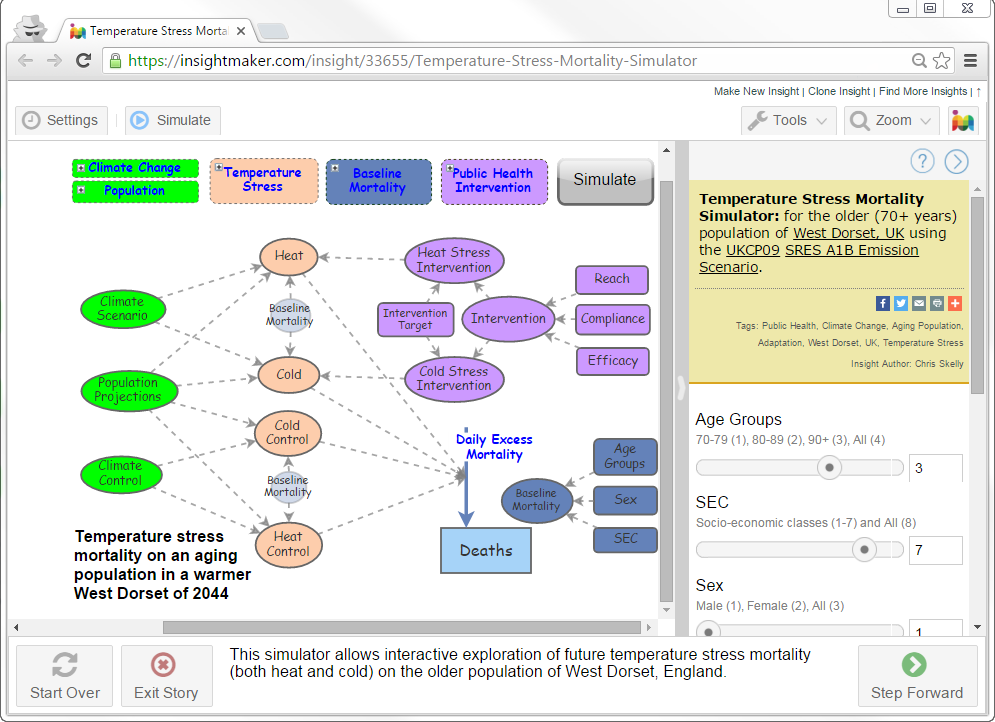
\includegraphics{./CCA/img/InsightMaker_GuestScreen.png}
	\caption[Insight Maker Guest Login Screen]{Users of our system model ``Temperature Stress Mortality Simulator'' will be presented with this user interface if they follow the provided link. Note that there are now more menu tabs along the top of the screen: add primitives, flows/transitions/links, edit, style. These tabs contain the tools for editing and creating models.\label{fig:IMGuest}}
\end{figure*}

\subsection{How to modify the model}
Follow this link: \href{https://insightmaker.com/}{Insight Maker}\sidenote{https://insightmaker.com/} to get to the page that allows participants to set up an account, explore other people's models and create your own (Figure~\ref{fig:IMLogin}).

\begin{description}
	\item [Create account] `Create a Free Account' -- top-right of screen
	\item [Search for Model] `Explore Insights' --> `Find Insights' --> `Search': Temperature Stress Mortality Simulator
	\item [Copy Model] Select model --> Clone Insight (top-right menu)\sidenote{You now have your own copy of the model and you can make any modifications to it that you like.}
\end{description}

\begin{figure*}[htbp]
	\centering
	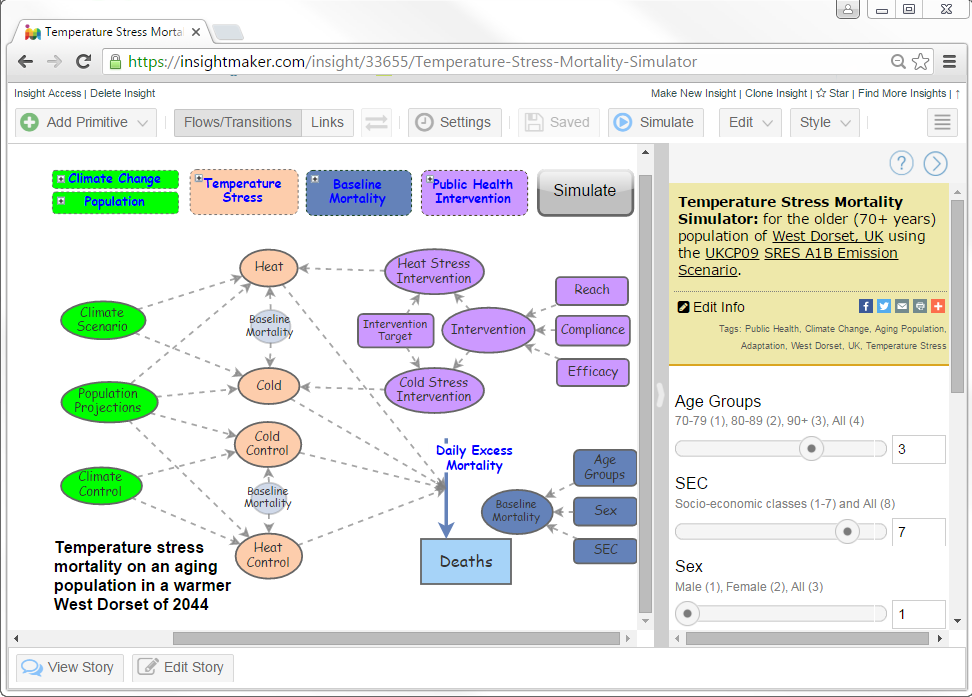
\includegraphics{./CCA/img/InsightMaker_LoggedinScreen.png}
	\caption[Insight Maker User Login Screen]{Users of our system model ``Temperature Stress Mortality Simulator'' will be presented with this user interface if they create a free account and make a copy of the model.\label{fig:IMLogin}}
\end{figure*}

\subsection{Story Telling} \label{section:modelstory}
The `model story' is an interactive tour of the system model developed for this project that was produced using \href{https://insightmaker.com}{Insight Maker}\sidenote{insightmaker.com/}. The story is available online allowing direct interaction with the model \href{https://insightmaker.com/insight/33655/Temperature-Stress-Mortality-Simulator}{Temperature Stress Mortality Simulator}\sidenote{insightmaker.com/insight/33655/ Temperature-Stress-Mortality-Simulator}.

By Chris Skelly\\
June 20, 2015
\begin{description}
	\item[Temperature Stress Mortality Simulator:] for the older (70+ years) population of~\href{http://en.wikipedia.org/wiki/West\_Dorset}{West Dorset, UK}\sidenote{en.wikipedia.org/wiki/West\_Dorset}~using the~\href{http://ukclimateprojections.metoffice.gov.uk/}{UKCP09}\sidenote{ukclimateprojections.metoffice.gov.uk}~\href{http://www.grida.no/publications/other/ipcc\_sr/?src=/climate/ipcc/emission/}{SRES A1B Emission Scenario}\sidenote{www.grida.no/publications/other/ ipcc\_sr/?src=/climate/ipcc/emission/}.
	\item[Acknowledgements] We would like to thank Communities Living Sustainably for funding this project from a Big Lotteries grant and all my colleagues at Dorset Public Health who made this project happen --- Chris Ricketts wrote the proposal and guided its early development, Rebecca Pearce managed the project and Dave Lemon undertook the modelling work to adapt temperature stress to West Dorset.
\end{description}

\begin{figure}[tb]
	\centering
	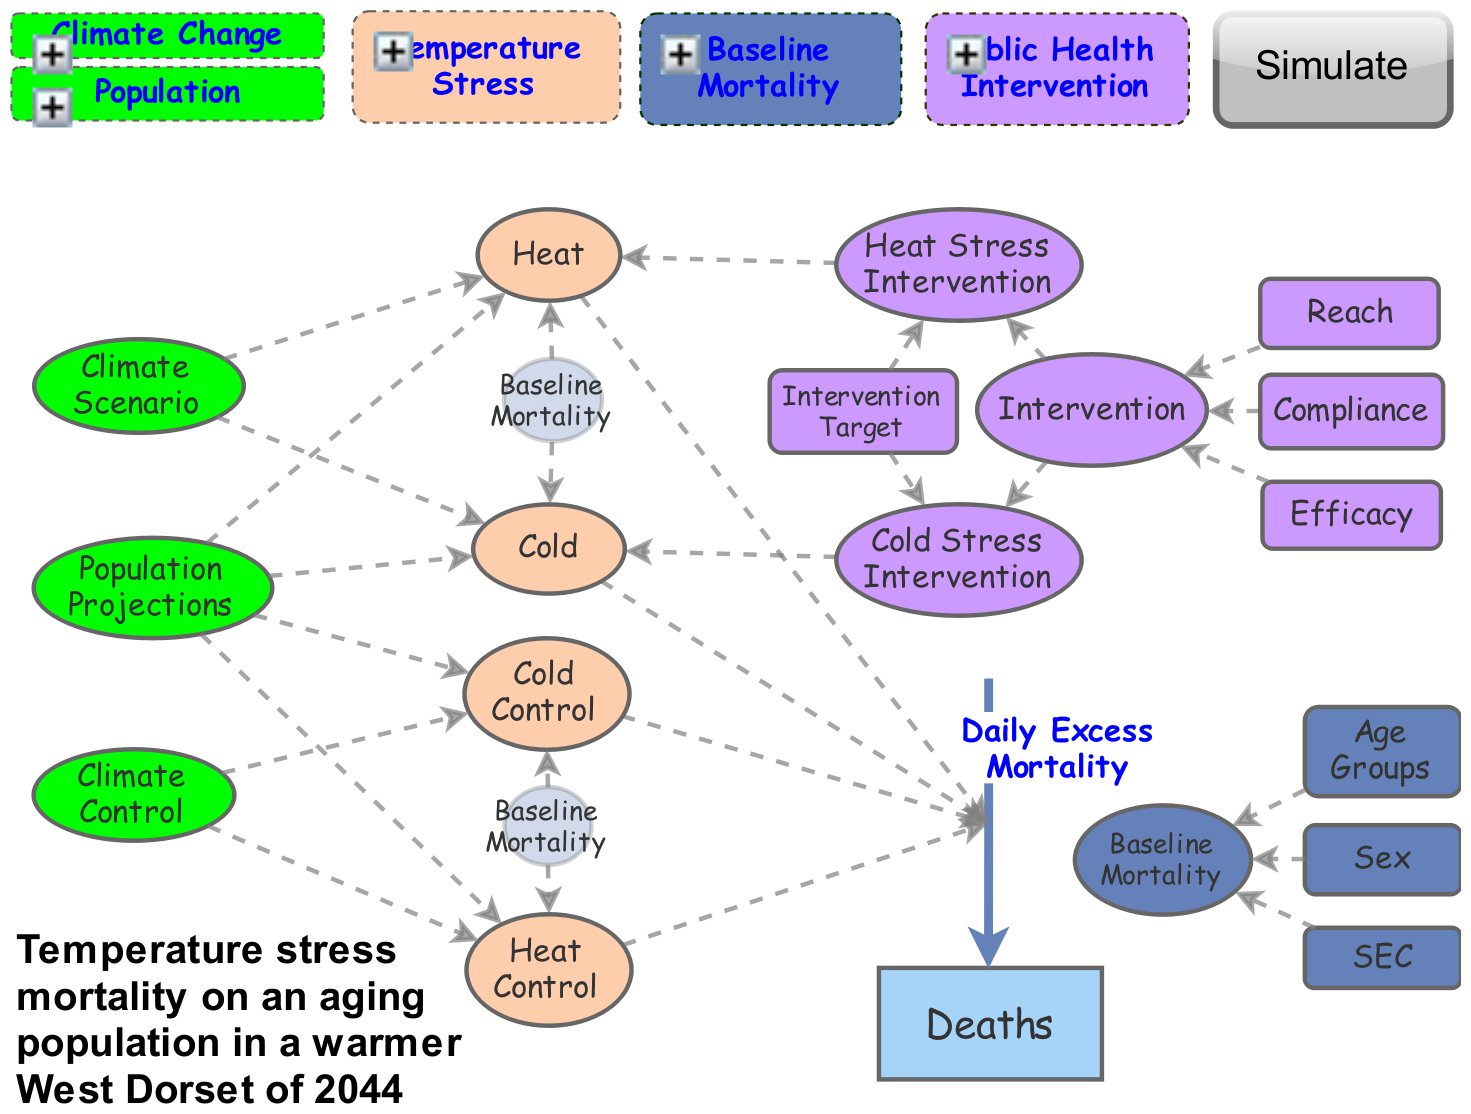
\includegraphics{./CCA/img/image_1.png}
	\caption[System Model Simulator]{This simulator allows interactive exploration of future temperature stress mortality (both heat and cold) on the older population of West Dorset, England.}
\end{figure}

\begin{figure}[htbp]
	\centering
	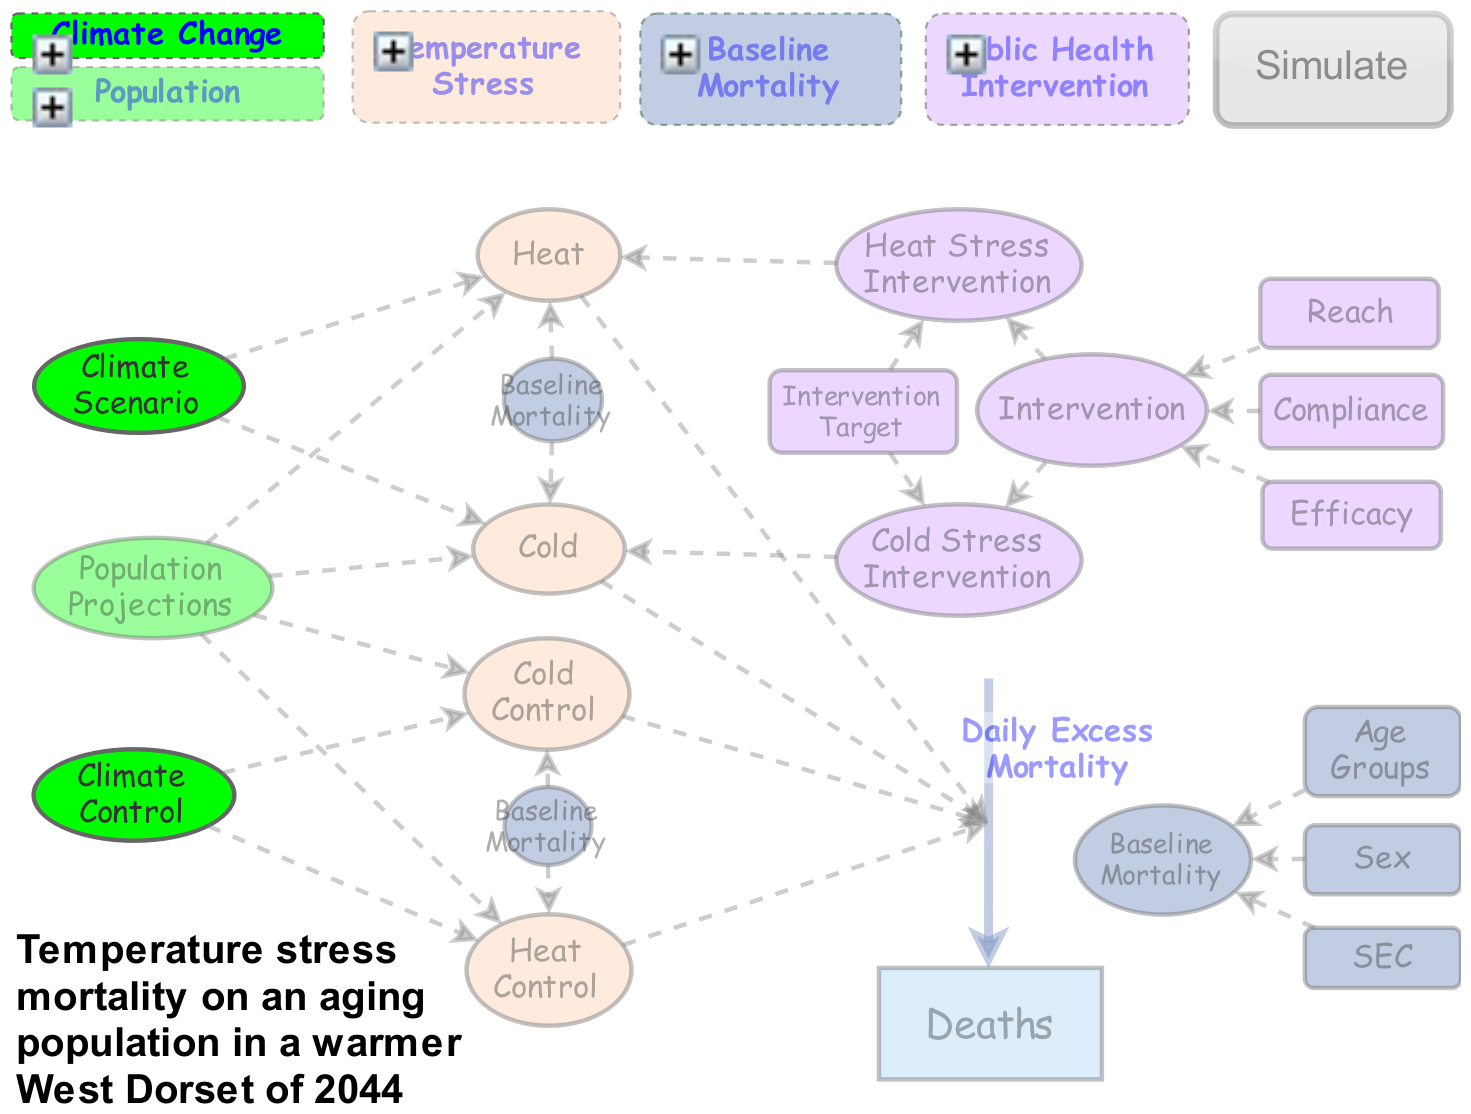
\includegraphics{./CCA/img/image_2.png}
	\caption[UKCP09 Scenario Data]{This simulator is driven using a future climate scenario (UKCP09) that is the basis of much climate adaptation policy in the United Kingdom. It is `downscaled' to the West Dorset region producing plausible daily temperature values for both the climate scenario (2044) and a control period (contemporary observed climate).}
\end{figure}

\begin{figure}[htbp]
	\centering
	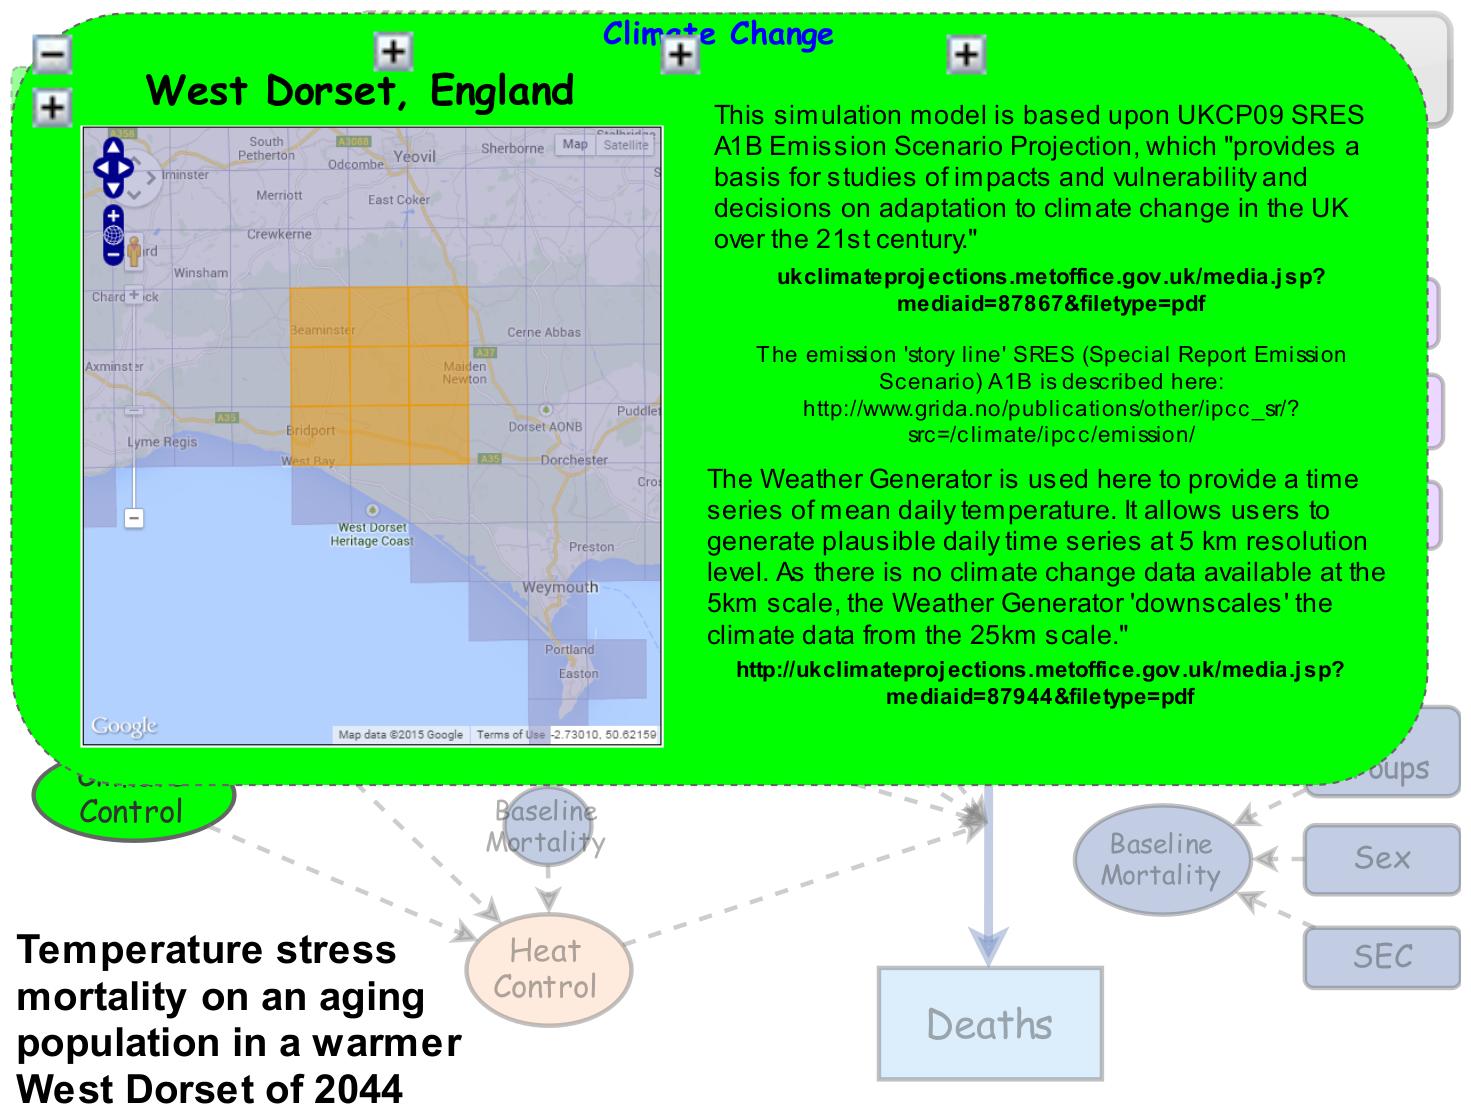
\includegraphics{./CCA/img/image_3.png}
	\caption[Simulated Climate Data]{Simulated climate data and scenarios details are found here.}
\end{figure}

\begin{figure}[htbp]
	\centering
	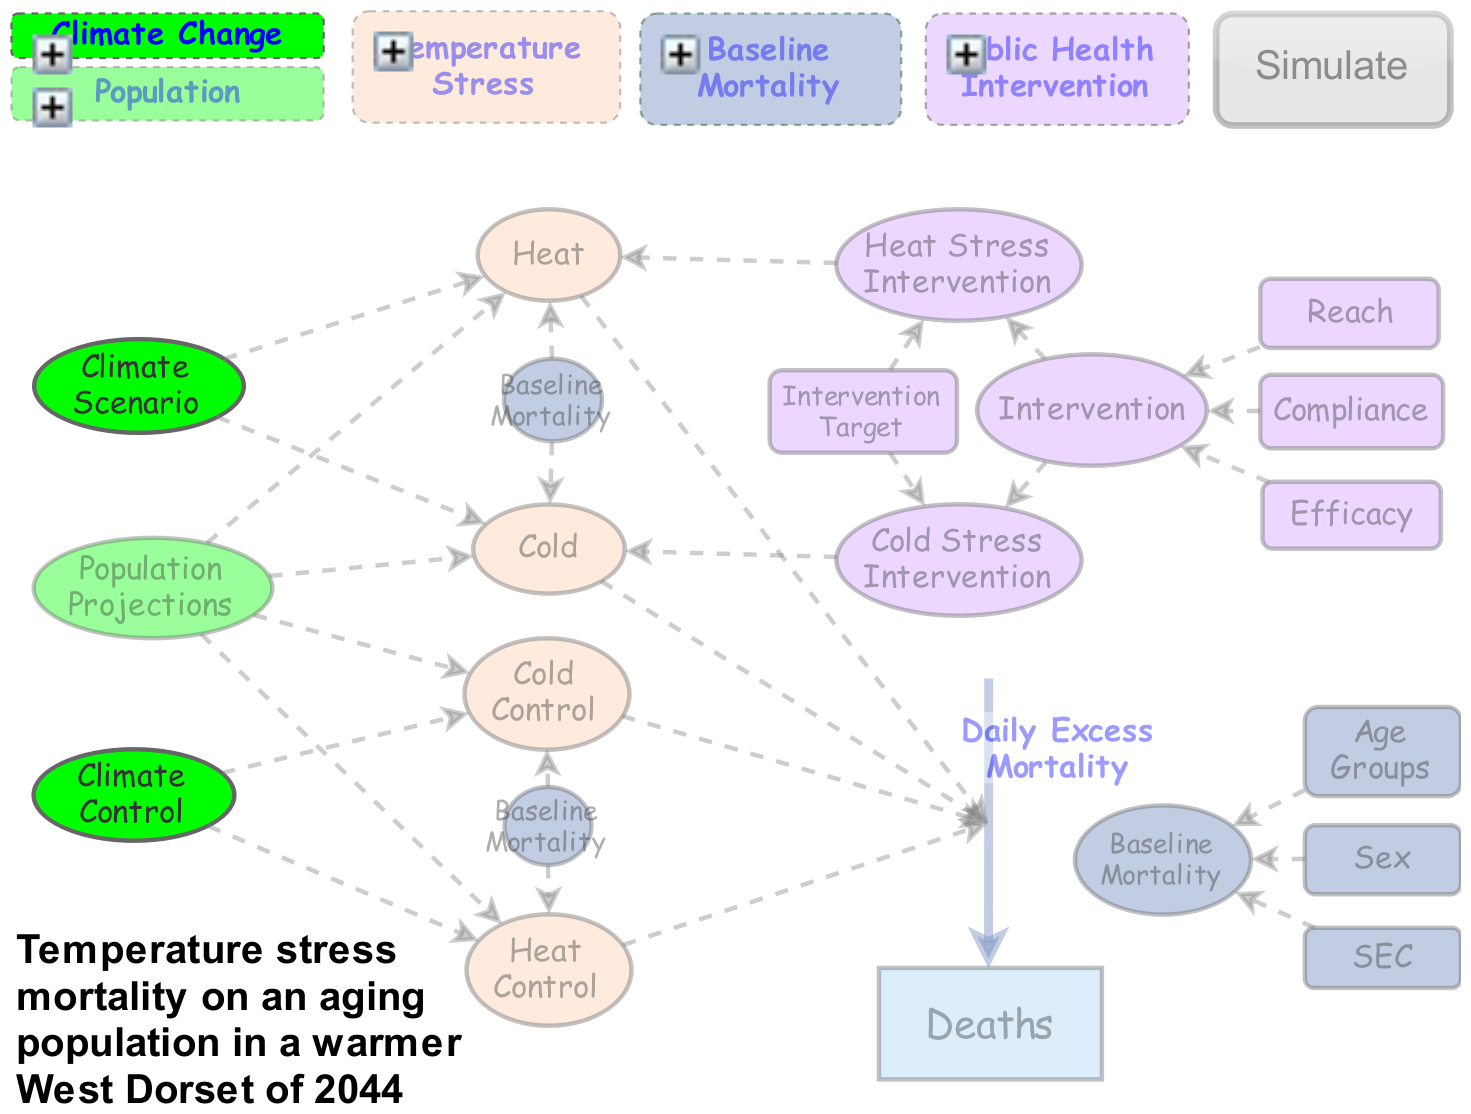
\includegraphics{./CCA/img/image_4.png}
	\caption[Population Change in West Dorset]{The climate is not the only thing that is forecast to change in West Dorset by 2044\ldots}
\end{figure}

\begin{figure}[htbp]
	\centering
	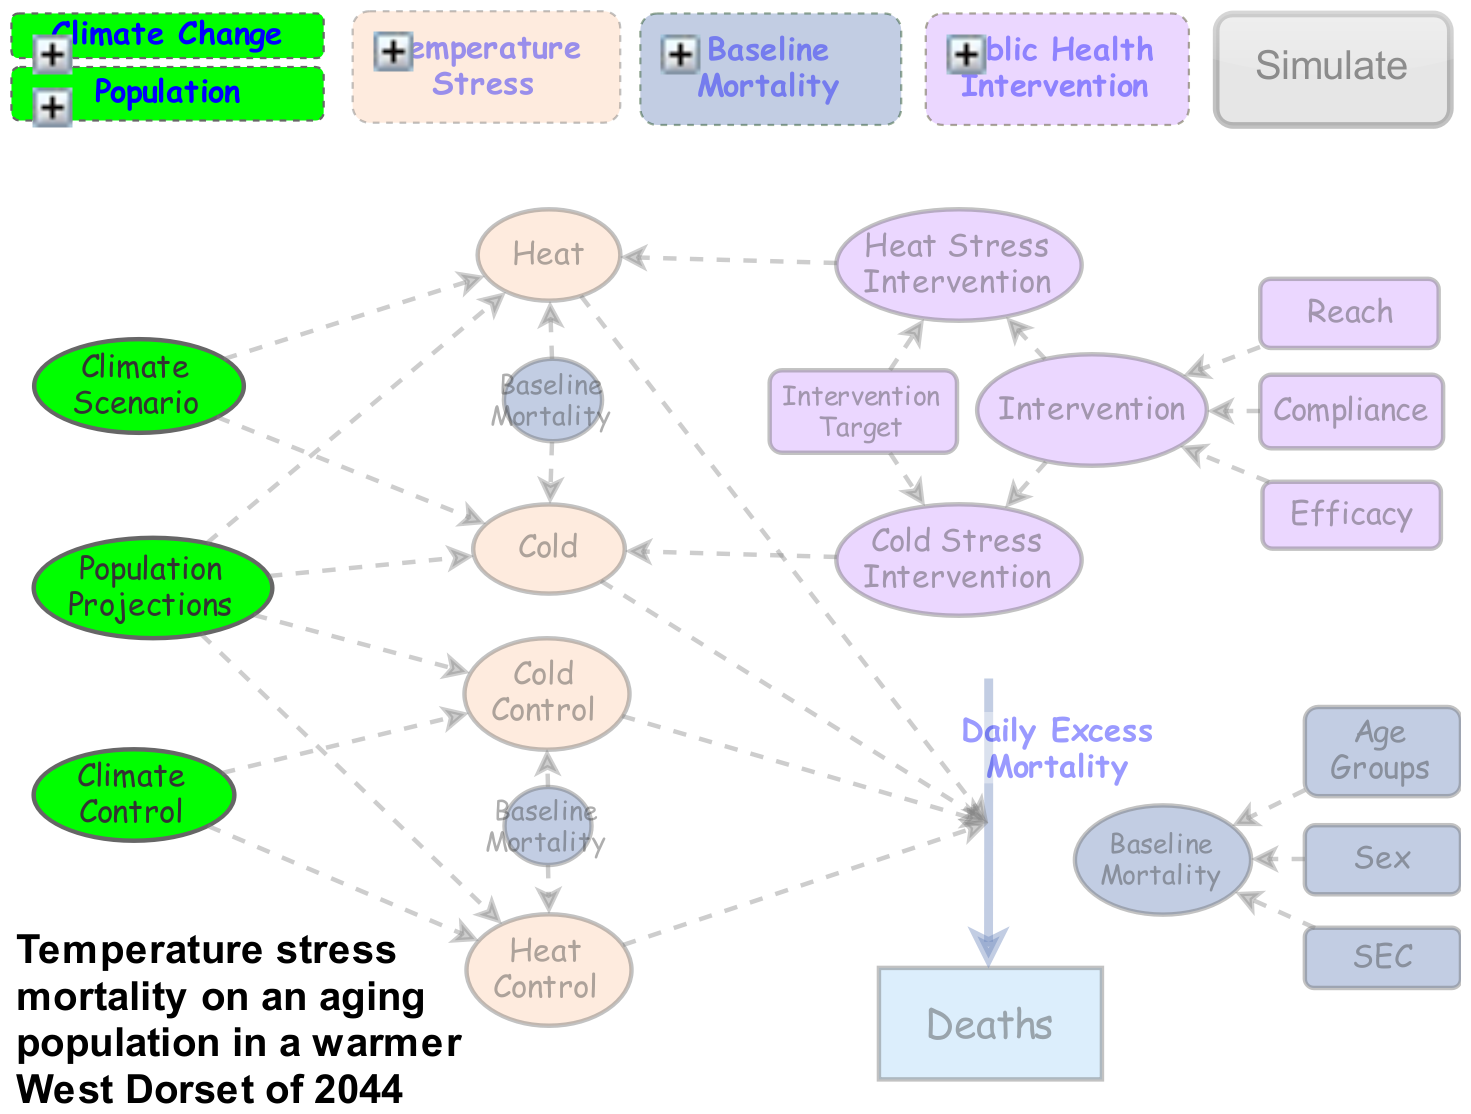
\includegraphics{./CCA/img/image_5.png}
	\caption[Ageing West Dorset Population]{The population of West Dorset, like that of the United Kingdom is ageing. In addition to an ageing population, there has been a retirement migration movement to the Dorset region for many years. This is likely to continue.}
\end{figure}

\begin{figure}[htbp]
	\centering
	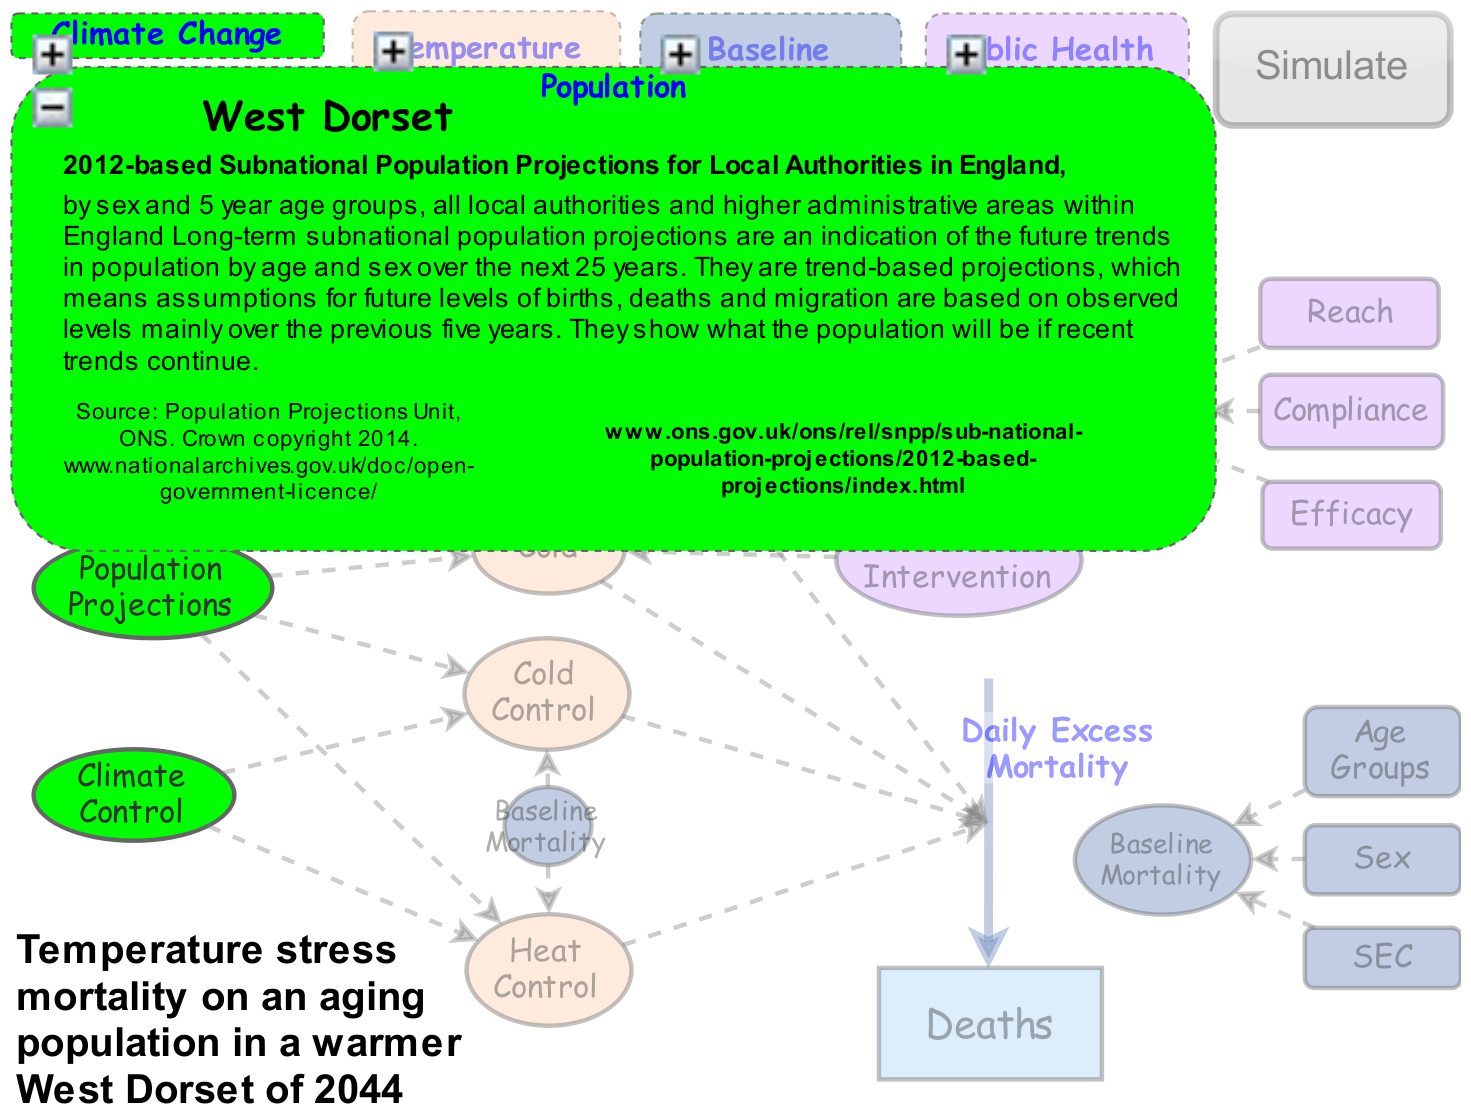
\includegraphics{./CCA/img/image_6.png}
	\caption[ONS Population Projections]{Population projection data, from the~Office of National Statistics, is detailed in this folder.}
\end{figure}

\begin{figure}[htbp]
	\centering
	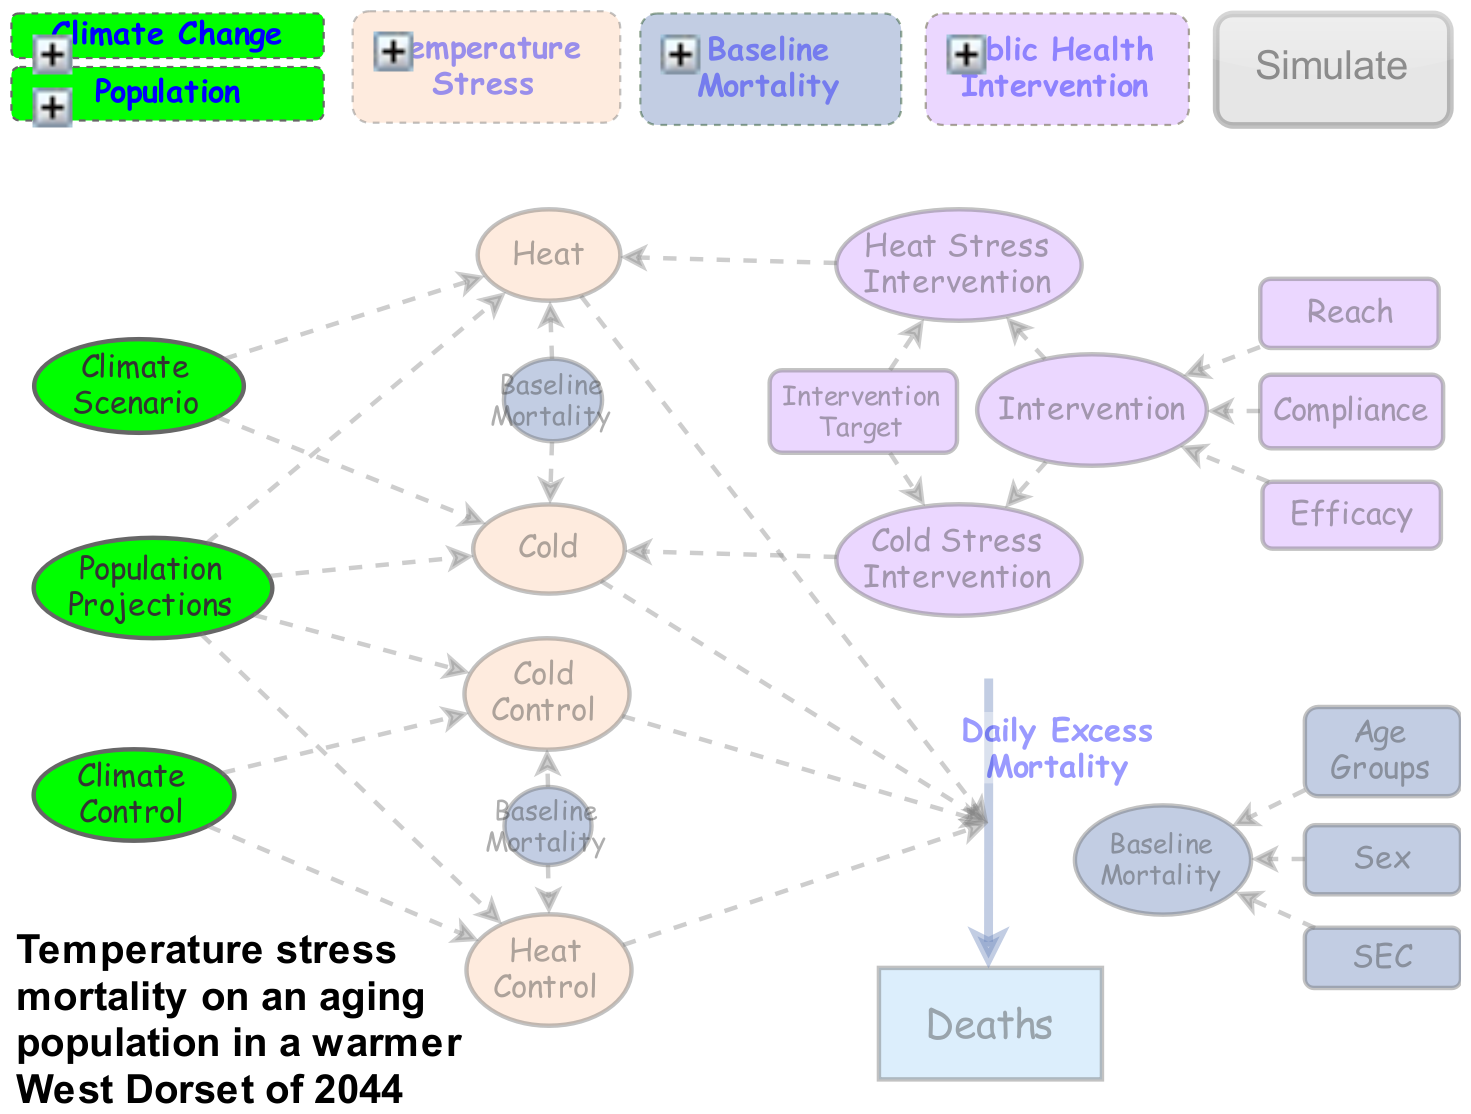
\includegraphics{./CCA/img/image_7.png}
	\caption[Climate Warming and Population Ageing]{The climate is expected to warm and the population is expected to age.}
\end{figure}

\begin{figure}[htbp]
	\centering
	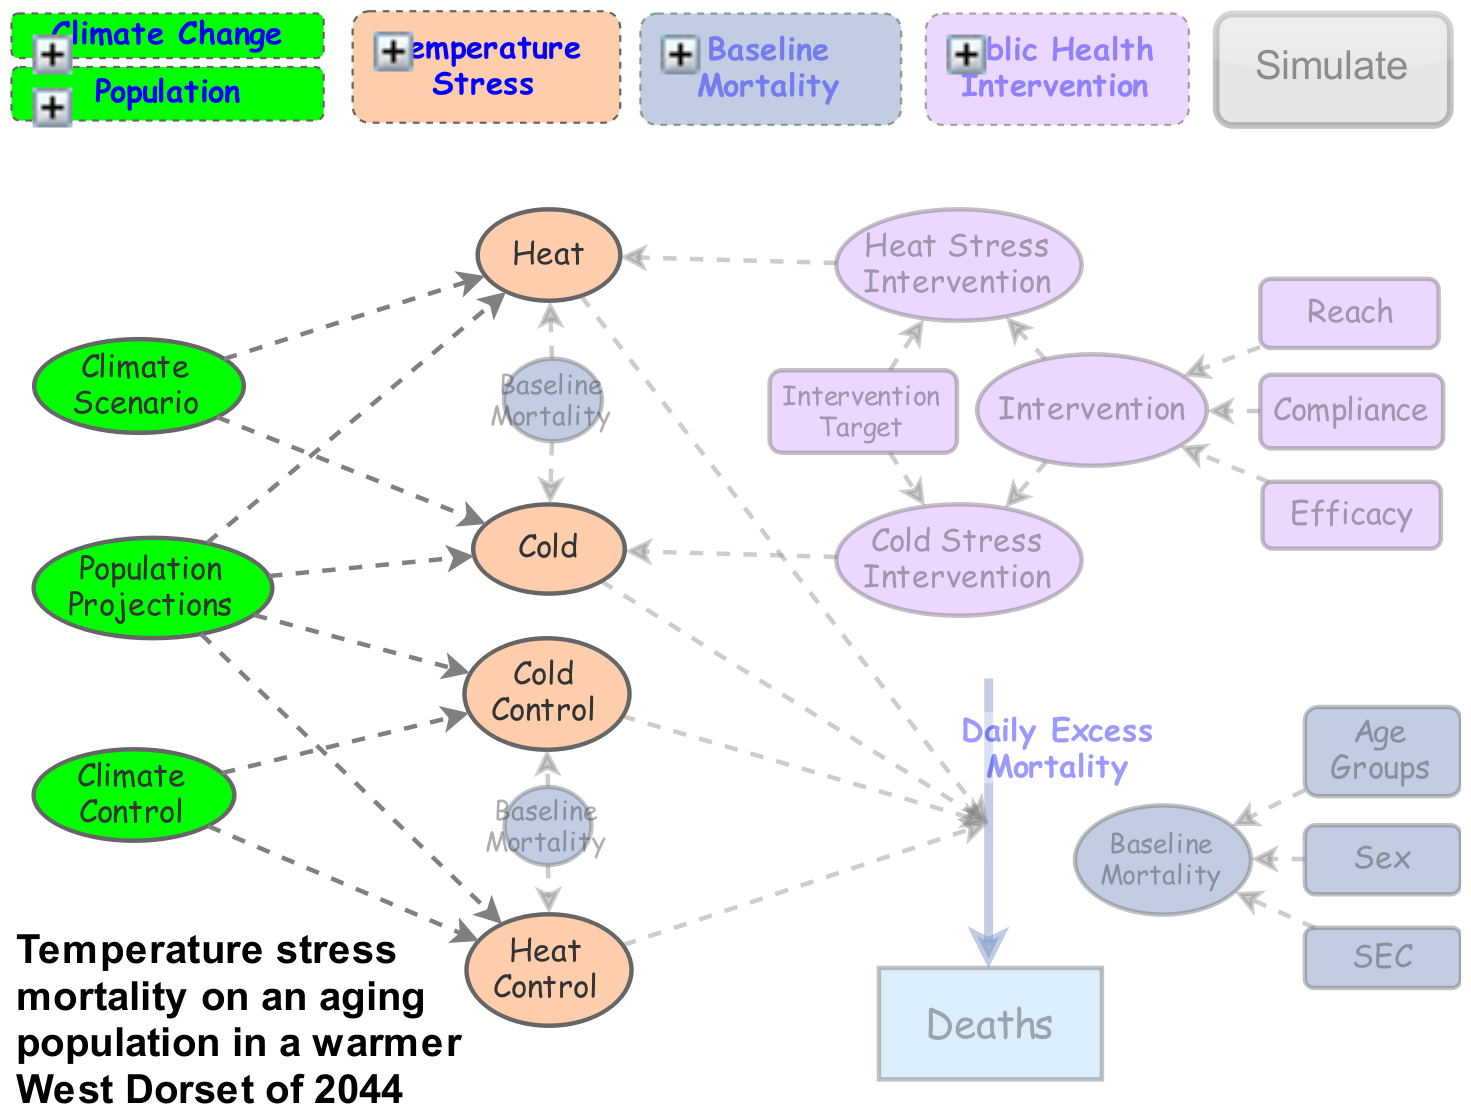
\includegraphics{./CCA/img/image_8.png}
	\caption[Thermal Stress]{Human physiology responds to ambient temperatures. If it is too warm or too cold the human body is stressed. This is most noticeable during major heatwaves when most of the population can feel the `heat stress'.}
\end{figure}

\begin{figure}[htbp]
	\centering
	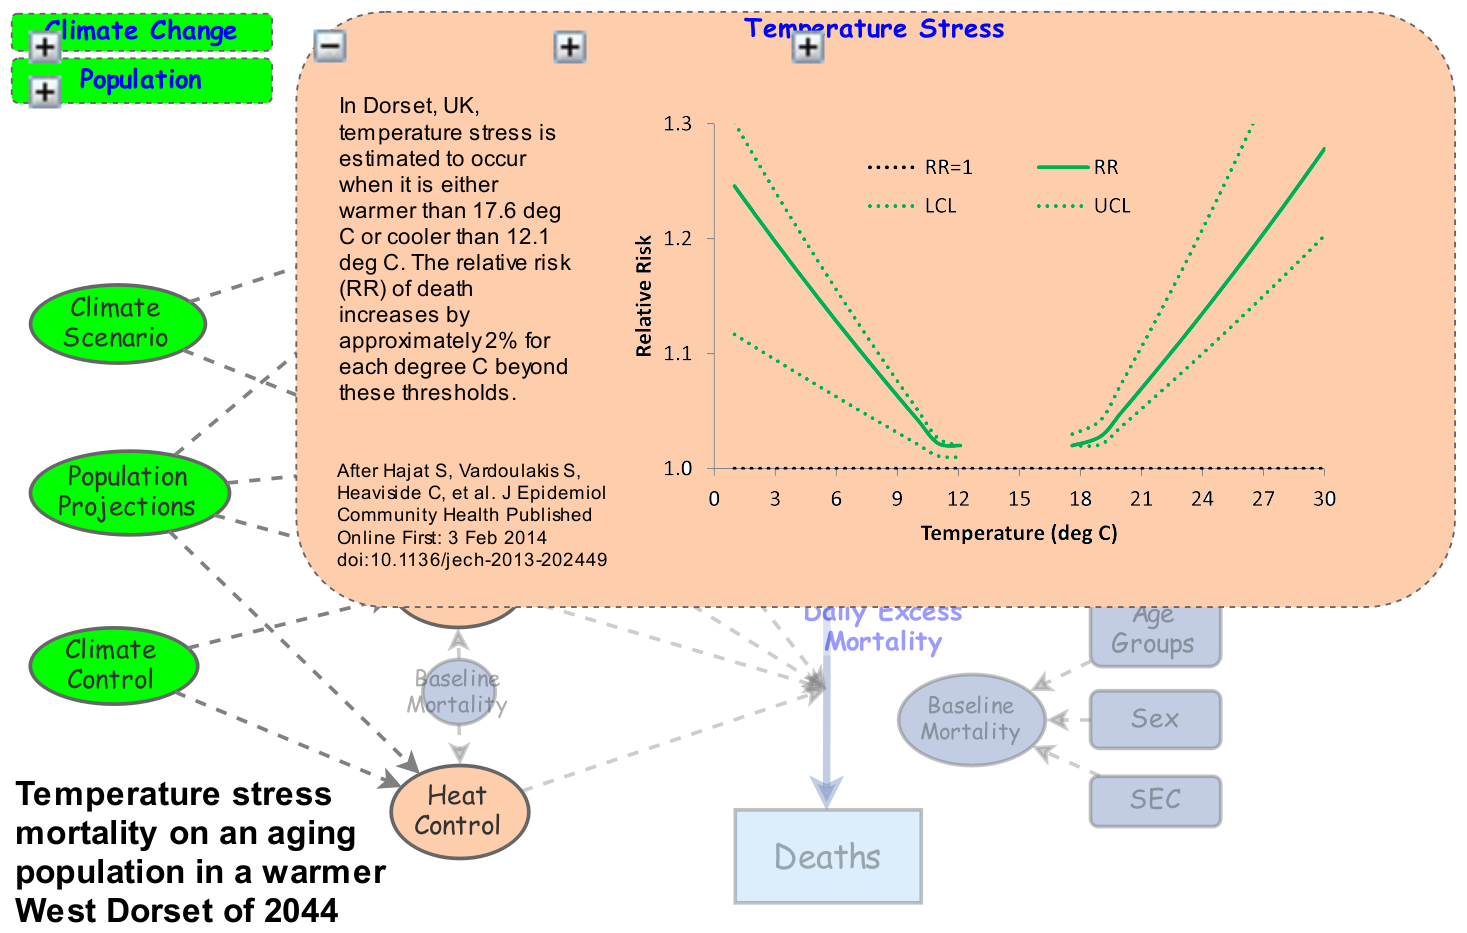
\includegraphics{./CCA/img/image_9.png}
	\caption[Thermal Stress Thresholds]{However, temperature stress occurs far more frequently than we might think -- and in Dorset at almost any time of year. Additionally, as we age, we tend to `feel' the cold or heat more. In other words, we experience more temperature stress. We have adapted a model that estimates the mortality associated with temperature stress in the West Dorset climate. It uses a `base mortality rate' (more on this later) for a population to estimate the temperature stress related `excess mortality'. This model shows that for every 1 degree C in temperature over either a heat or cold threshold excess mortality increases by 2\%. This is the fundamental relationship upon which this simulator is based.}
\end{figure}

\begin{figure}[htbp]
	\centering
	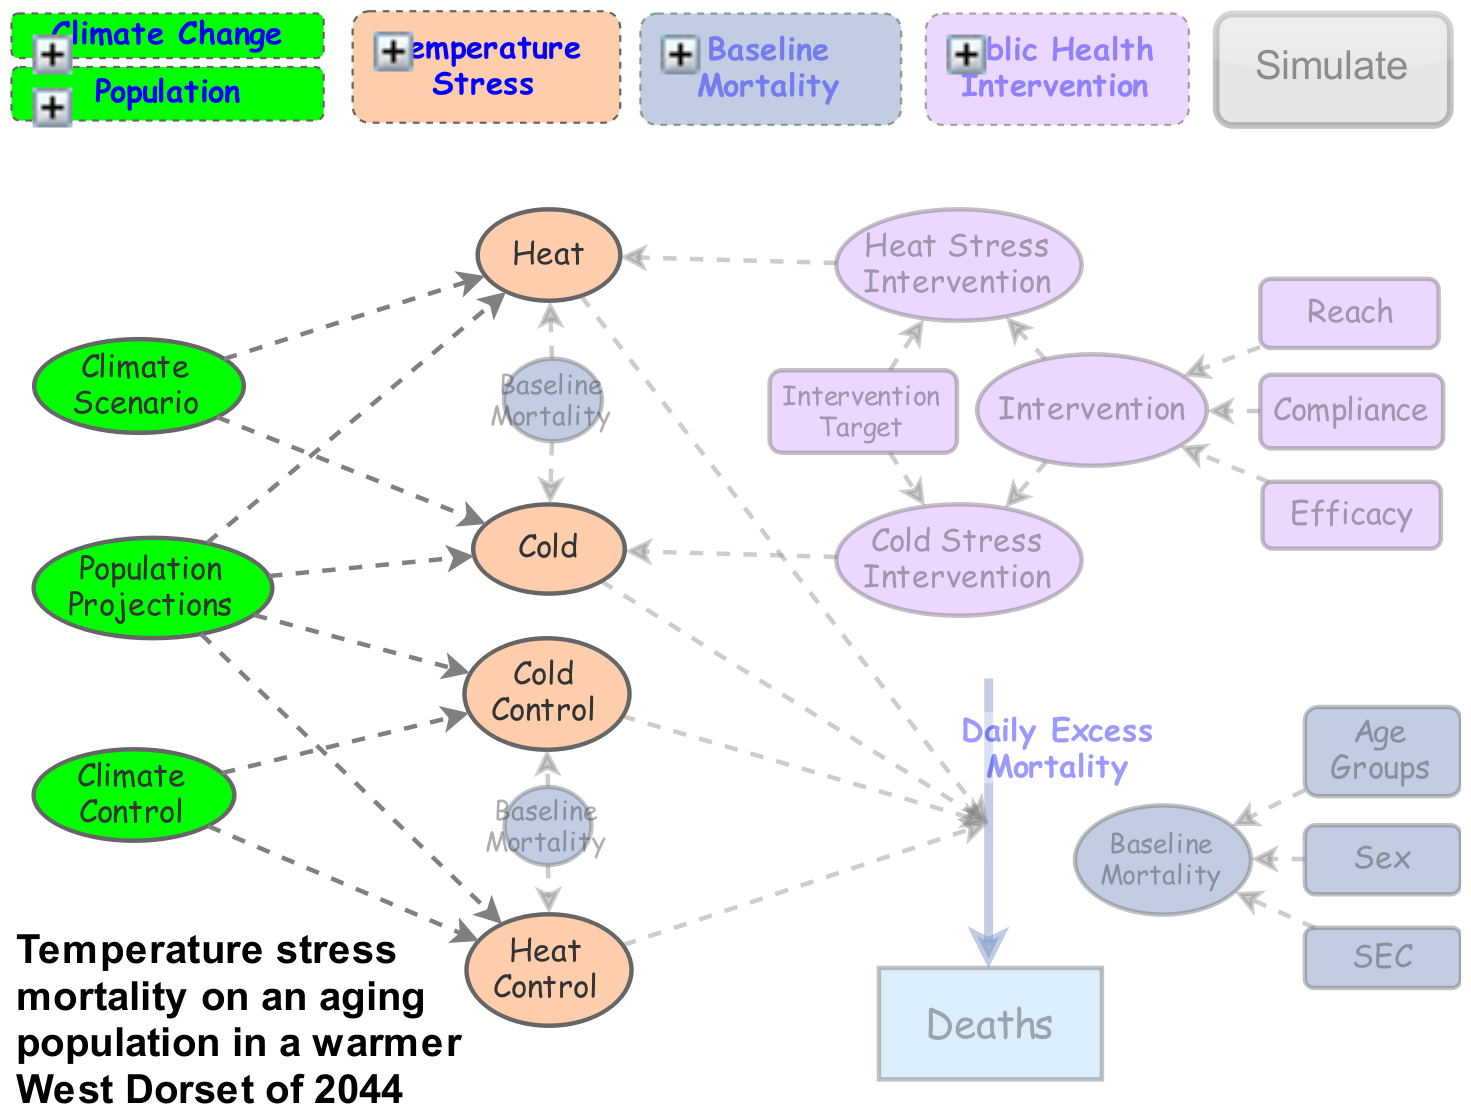
\includegraphics{./CCA/img/image_10.png}
	\caption[Base Mortality Rates]{The relationship between temperature and the base mortality rate is how we define `temperature stress'. But where do these `base mortality rates' come from?}
\end{figure}

\begin{figure}[htbp]
	\centering
	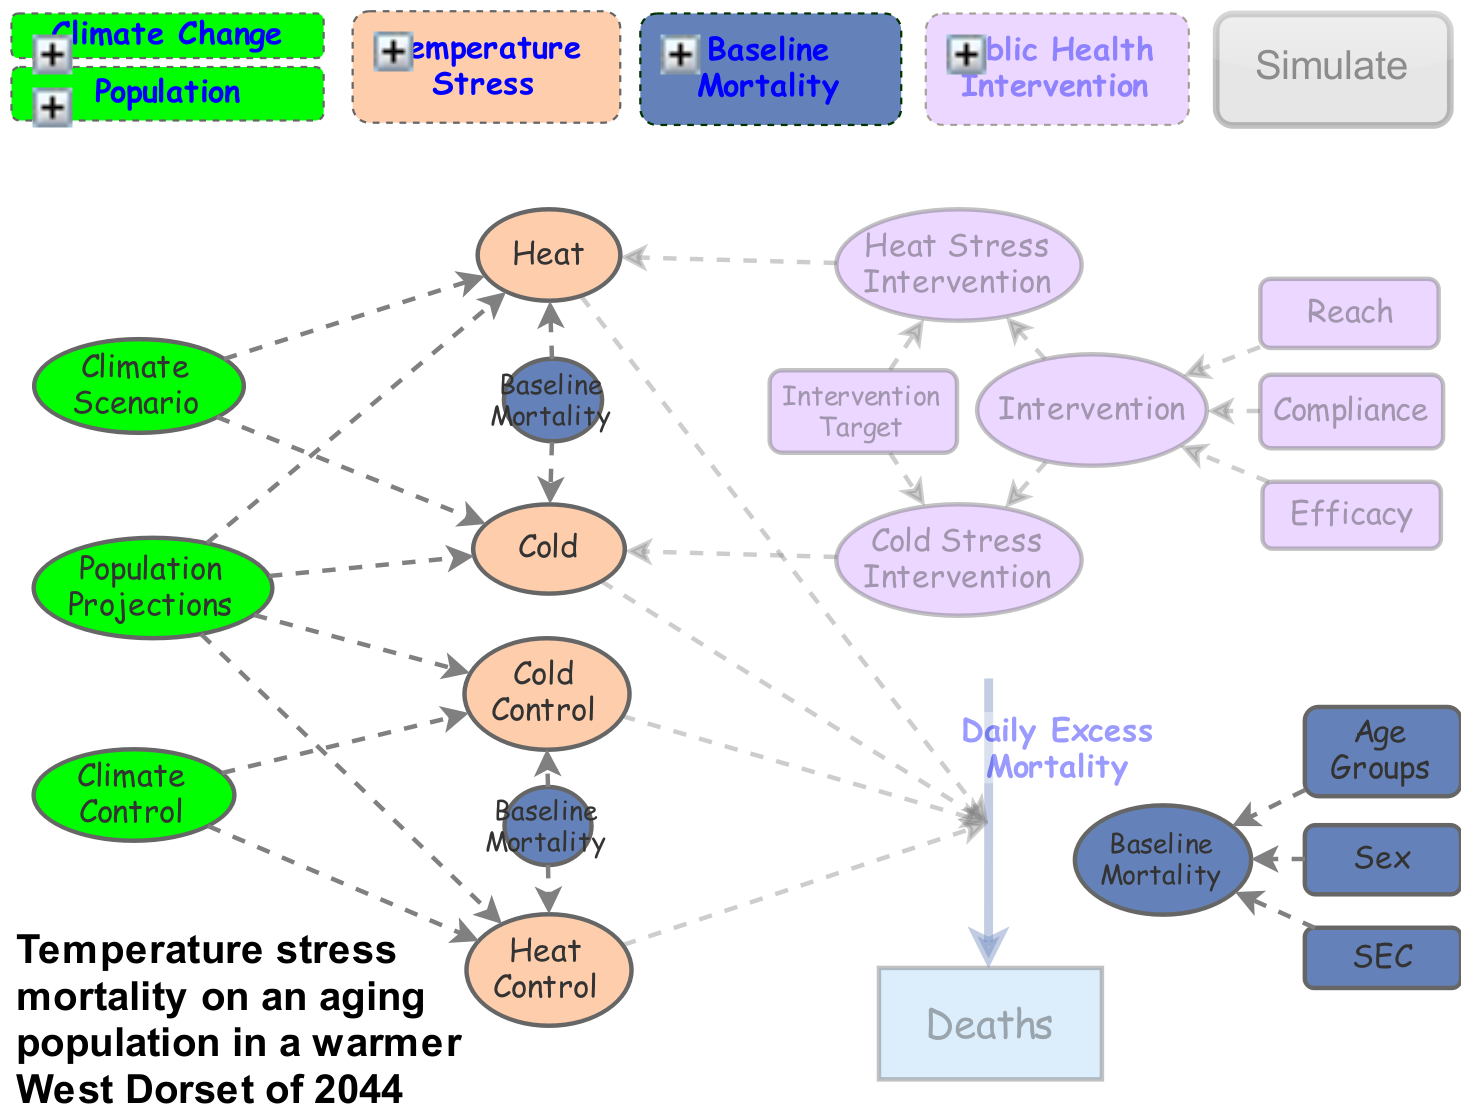
\includegraphics{./CCA/img/image_11.png}
	\caption[Age Specific Base Mortality Rates]{Base mortality rates are produced in the United kingdom for different groups by age, gender and socio-economic class (SEC), because it is well established that there are significant inequalities across these groups.}
\end{figure}

\begin{figure}[htbp]
	\centering
	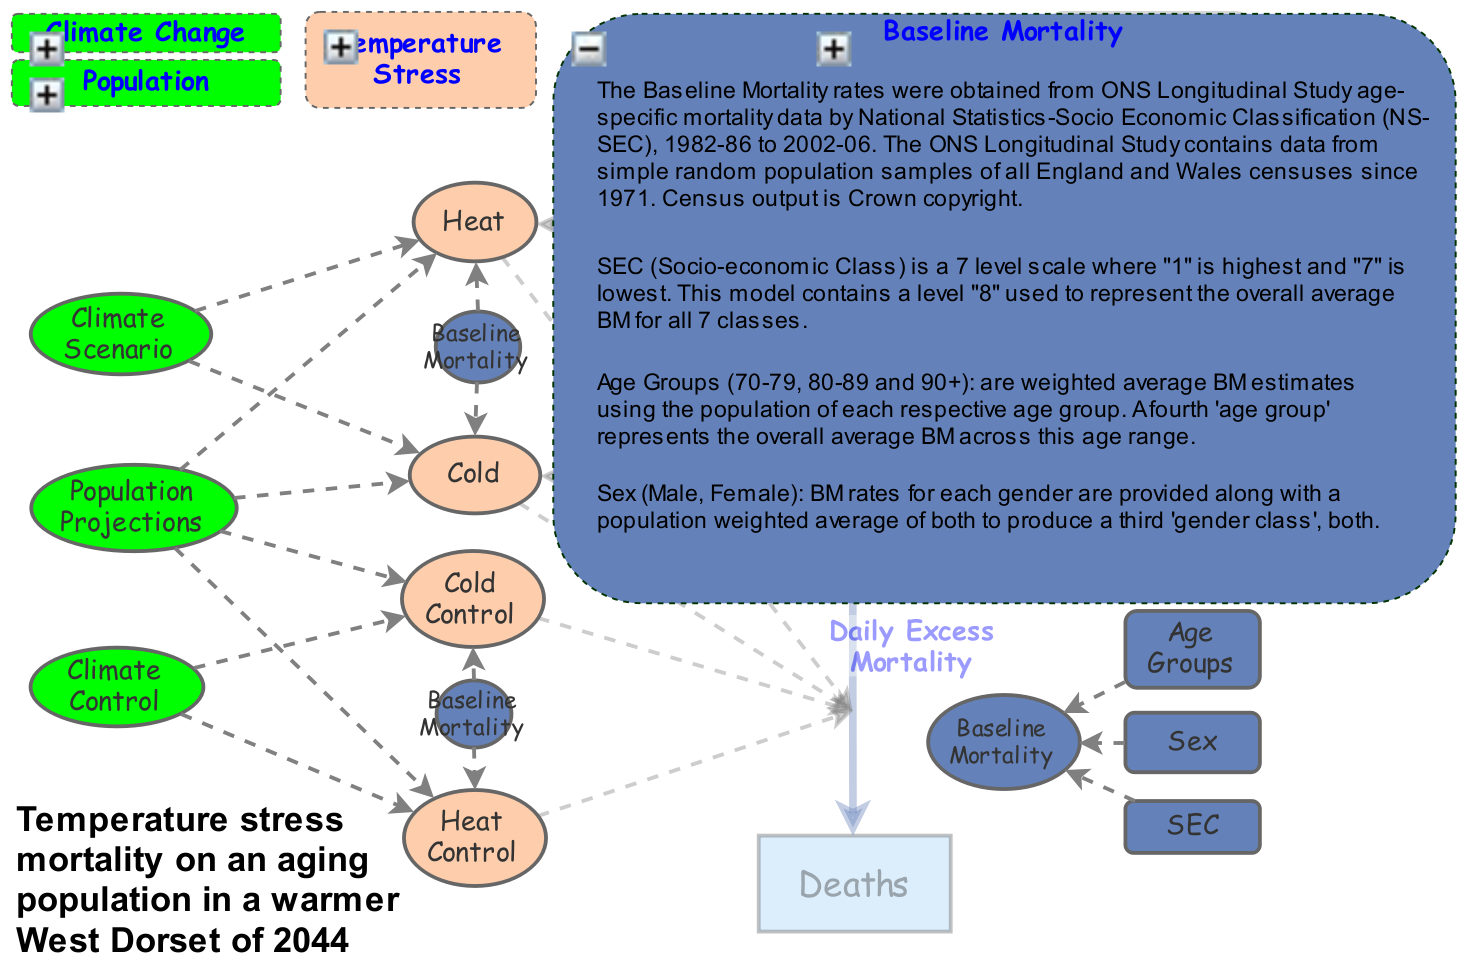
\includegraphics{./CCA/img/image_12.png}
	\caption[Population Variables]{This simulator allows the user to set the age group (4 groups for the over 70+ population are available), sex and socio-economic class (SEC 1-7 is from highest to lowest and 8 is for all classes).}
\end{figure}

\begin{figure}[htbp]
	\centering
	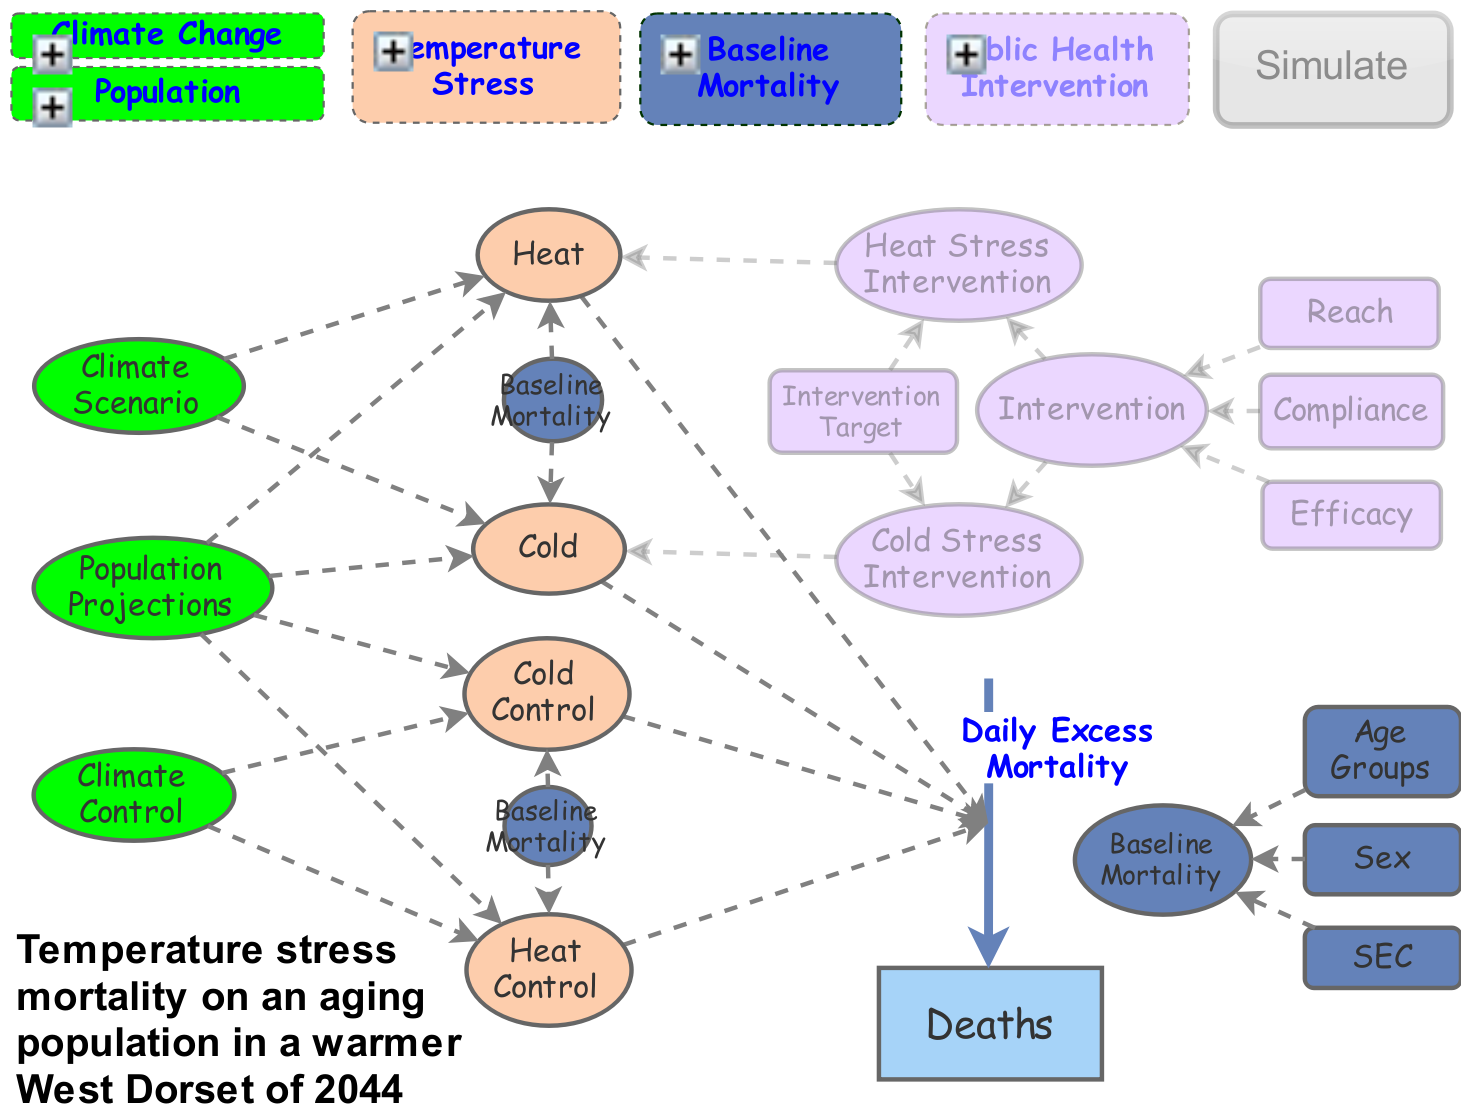
\includegraphics{./CCA/img/image_13.png}
	\caption[Cold Stress Excess Mortality is Higher]{It is worth noting at this point that even in a warmer West Dorset of 2044, mortality from cold stress will still be much higher than mortality from heat stress. Counter intuitive perhaps, but true. Of course excess mortality due to cold stress will be lower in the future (although still much higher than heat stress). More on this later -- it has implications for public health interventions. There are four `daily excess mortality' values estimated: excess mortality from future heat and cold stress and for comparison `control excess mortalities' are also estimated.}
\end{figure}

\begin{figure}[htbp]
	\centering
	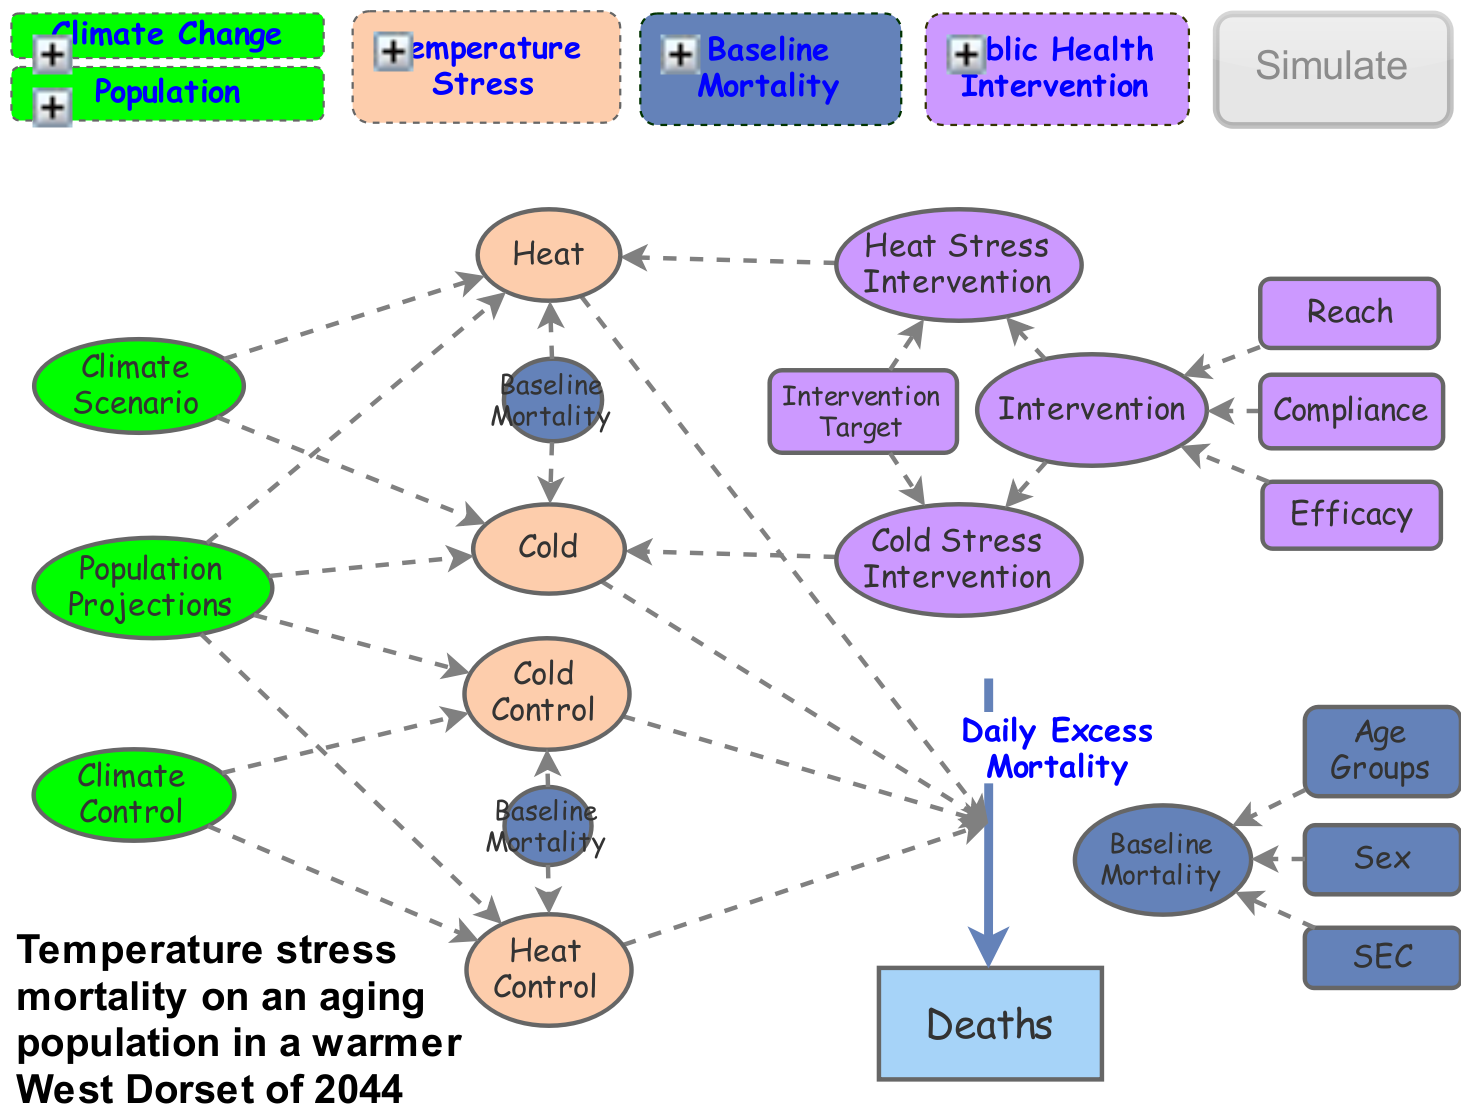
\includegraphics{./CCA/img/image_14.png}
	\caption[Devising Public Health Interventions]{You can compare these sources of excess mortality as they accumulate over the simulation period.So what public health interventions might be taken in order to assist the target population in adapting to more heat stress?}
\end{figure}

\begin{figure}[htbp]
	\centering
	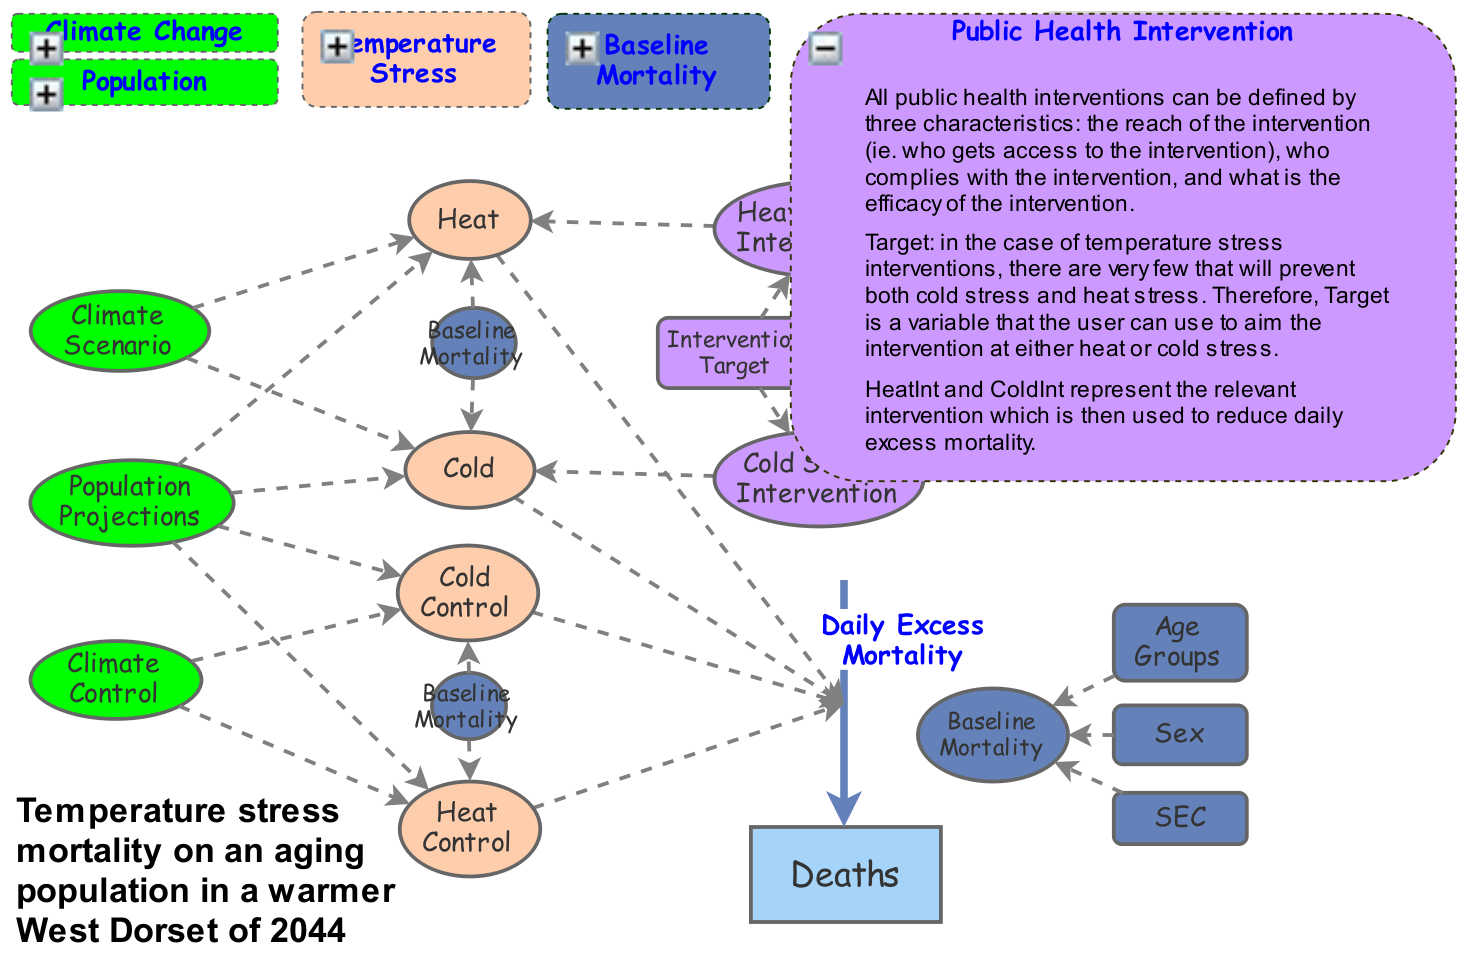
\includegraphics{./CCA/img/image_15.png}
	\caption[Intervention Targeting Options]{You have the option of trialling an intervention for either heat or cold stress, but not both at the same time. The default setting is for NO intervention. `Intervention Targeting' is the variable used to set which intervention will be made.}
\end{figure}

\begin{figure}[htbp]
	\centering
	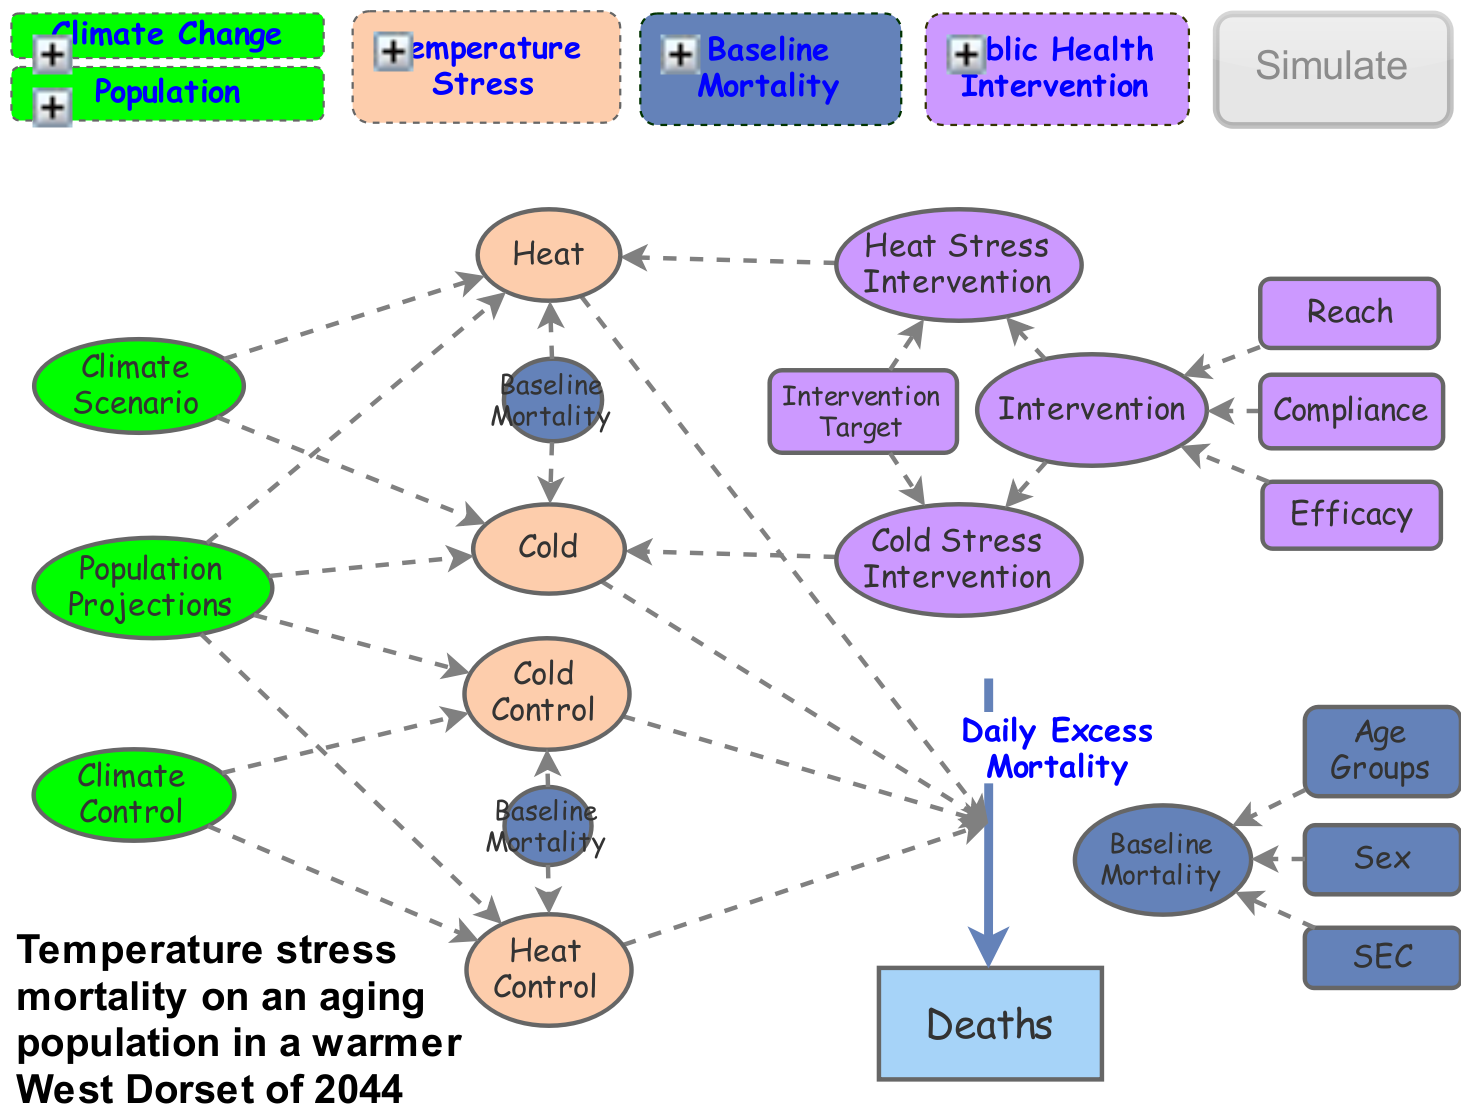
\includegraphics{./CCA/img/image_16.png}
	\caption[Elements of a Public Health Intervention]{All public health interventions have three basic variables: the proportion of the target population you can reach, the proportion of the population that comply with the intervention and the efficacy (how effective it is at doing what it is supposed to do) of the intervention.}
\end{figure}

\begin{figure}[htbp]
	\centering
	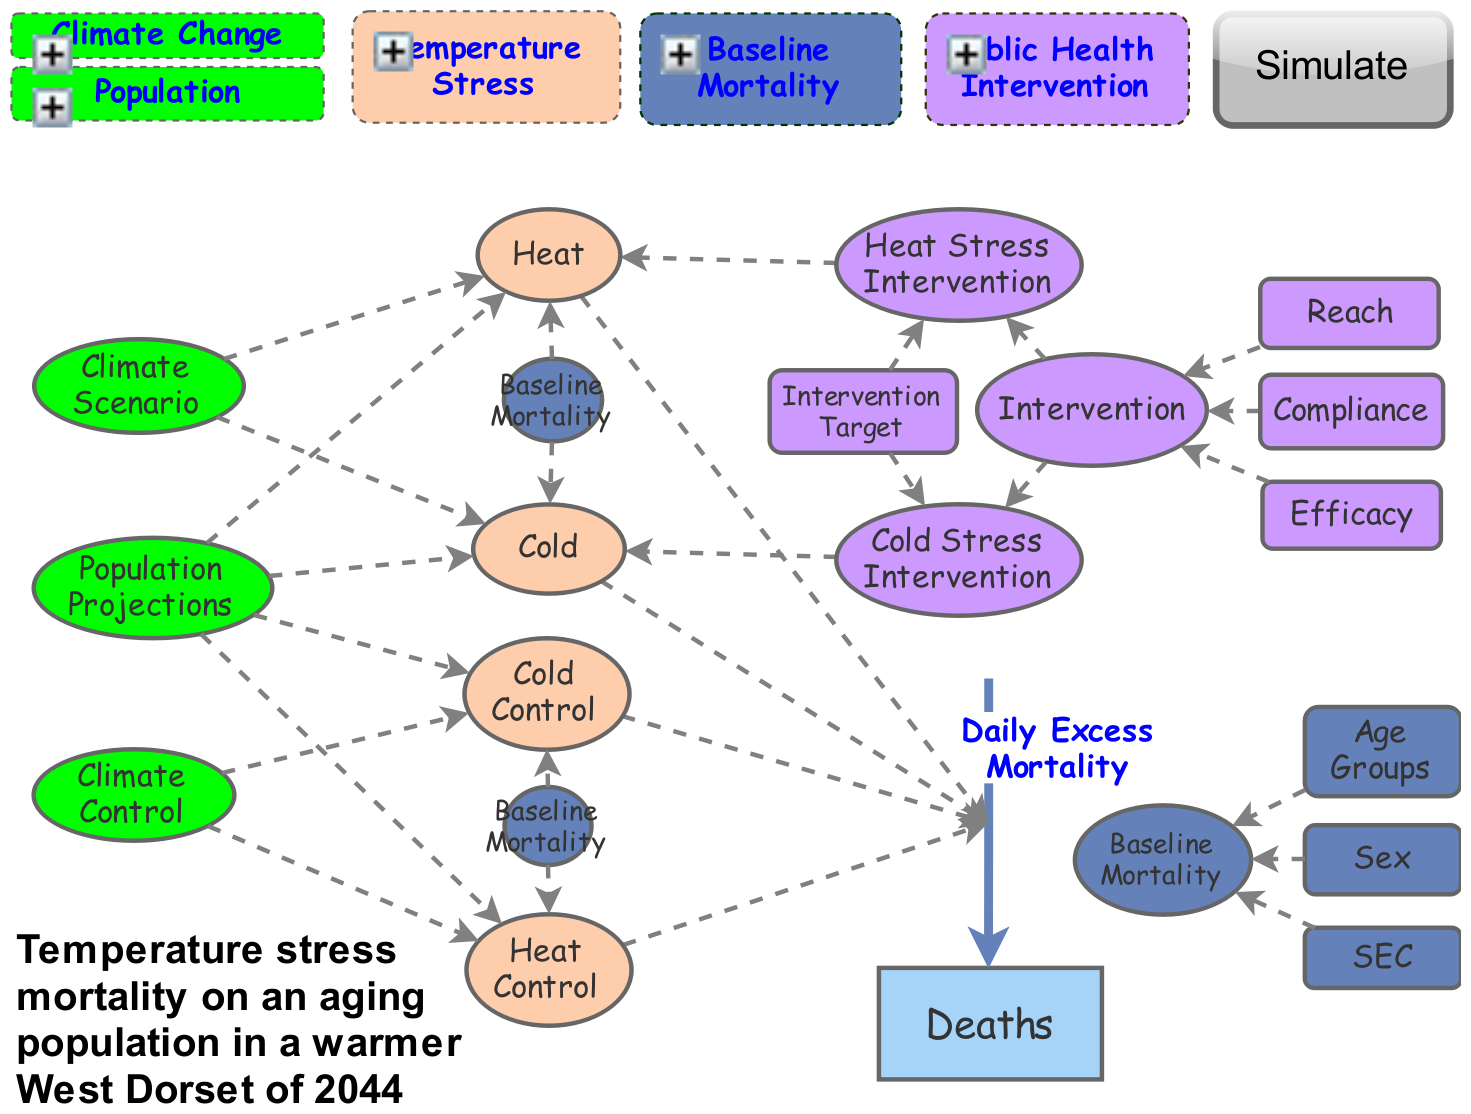
\includegraphics{./CCA/img/image_17.png}
	\caption[Run Simulation]{This `simulate' button produces the default simulation for a population with all age groups, all socio-economic classes and all both sexes included as a single population. Additionally, there are 10 years of simulated temperature data available (this default simulation setting uses the first 365 days). However, the `Settings' button at the top of the window allows the user to set the start and duration of the simulation period. The user will be presented with two daily excess mortality graphs (one for the future and one for the control), a combined accumulated deaths (both future and control) and a table of accumulated deaths.}
\end{figure}

\begin{figure}[htbp]
	\centering
	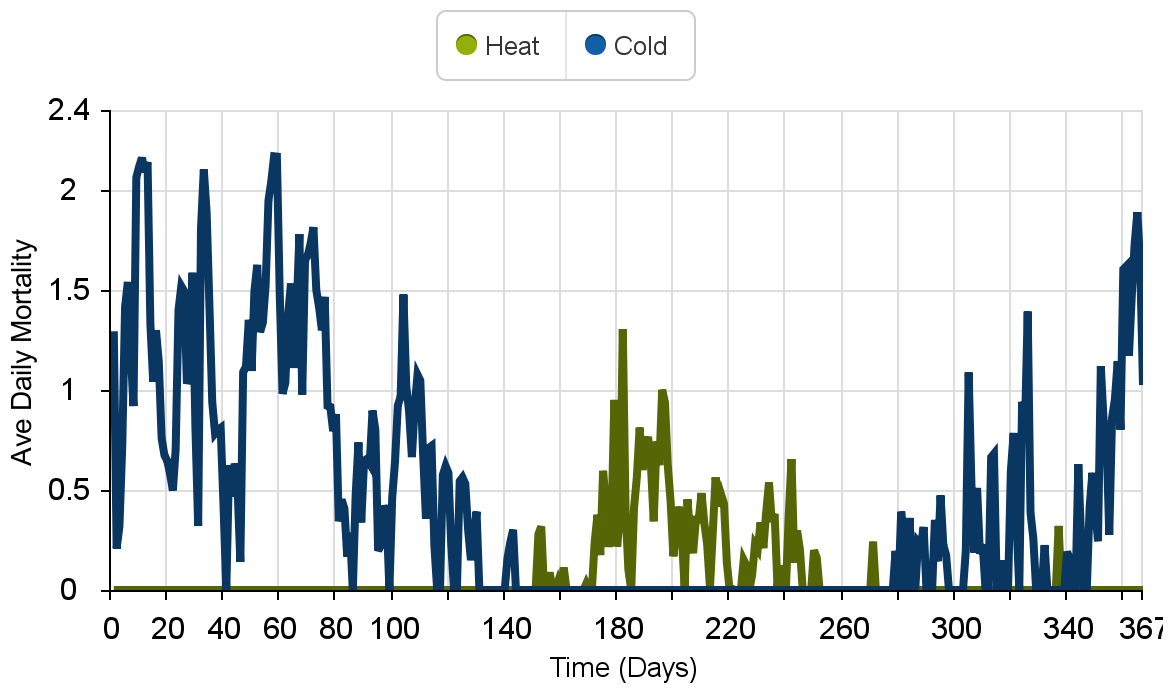
\includegraphics{./CCA/img/image_18.png}
	\caption[Simulation Output]{Do you see the three graph `tabs' above the graph? You can move between the visuals during the simulation. You can change the speed of the simulation and rerun it. The introduction to this model is now complete. You can `Exit Story' (bottom left of screen) and explore the model, its variables and its construction at your own pace. If you are unfamiliar with the Insight Maker modelling environment, you may wish to further explore that -- all models are open source -- set up your own free account to copy and modify this or any model for your own use and share with colleagues.}
\end{figure}



% Section 3 Futures Thinking
\section{Applications of Futures Thinking}
\label{horizonscanning}

\subsection{Introduction}
Futures thinking is...

This is a section to introduce futures thinking as a subtopic of systems thinking

Also called foresight

\subsection{Horizon Scanning}
Although, horizon scanning\cite{WikipediaFT} was essential to the development of future scenarios and the writing of a futures story, it was not made accessible outside of the project team and participants in our workshops. There were a couple reasons for this, the first was that we had very limited scope within the project to engage with the public and therefore limited our engagement to the futures story and secondly, the format produced by the horizon scanning tools was fairly rough and would be a lot of work to devise a method of communicating this directly.


During 2014, active horizon scanning was undertaken using the \url{http://www.shapingtomorrow.com/} web site. Membership is free and the site has numerous tools to enable future studies.

\begin{marginfigure}
	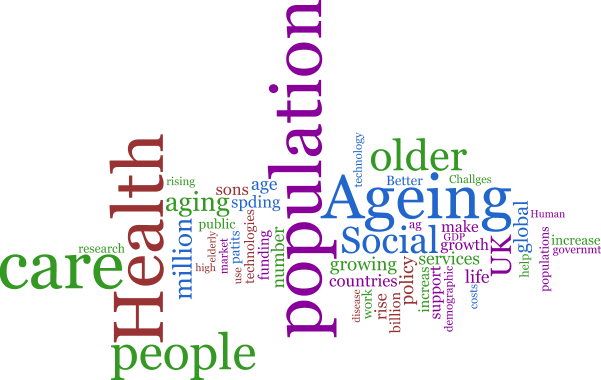
\includegraphics{CCA/img/FutureOlderPersonsWordCloud.png}
	\caption{Word cloud visualisation of horizon scanning results}
	\label{fig:wc}
\end{marginfigure}

What follows are the automatically derived insights generated by the Shaping Tomorrow tools from articles that were collected and run through their process. These tools are still in development and some of the automatically generated text is formatted poorly and/or grammatically incorrect due to the method used to extract the text (Figures~\ref{fig:wc}~and~\ref{fig:imap}).

\begin{figure*}
	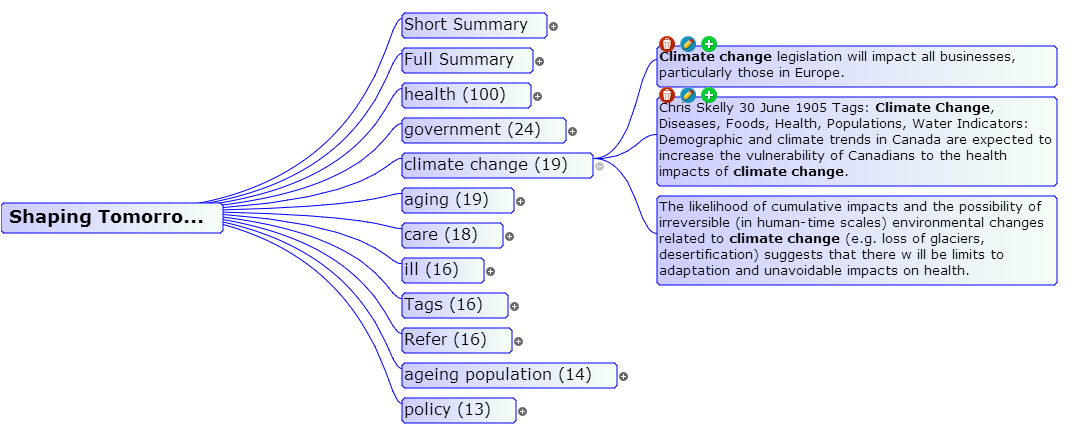
\includegraphics{CCA/img/WebSummarizerClimatechange.png}
	\caption[Shaping Tomorrow Tools]{A number of tools within Shaping Tomorrow's horizon scanning provide visual mapping of the results.}
	\label{fig:imap}
\end{figure*}

\begin{itemize}
	\item A lack of large-scale societal support programs for older populations in some Asian countries will be a major challenge for governments.
	\begin{quotation}
		Reflecting long-held ideas of functional foods derived from traditional medicines, Asia is the leading market for nutraceuticals.126 ? In 2010, China became the world's largest nutraceutical market.127 Implications and opportunities to 2040 The ageing of East Asia will happen much more rapidly than the ageing of the US and Europe; hence, East Asia will be forced to adapt more rapidly. A lack of large-scale societal support programs for older populations in some Asian countries will be a major challenge for governments.
	\end{quotation}
	\item Retraining and continuous learning will be at a premium and retirement policy will change dynamically.
	\begin{quotation}
		Climate change legislation will impact all businesses, particularly those in Europe. Energy and debt will remain important influencers of government policy for the coming decade. With less new foreign talent and more older workers, retraining and continuous learning will be at a premium and retirement policy will change dynamically.
	\end{quotation}
	\item Losing the smartest talent to more attractive economies will hamper R\&D and innovation.
	\begin{quotation}
		Consumers and employees are becoming older and more ethnically diverse in many European markets. Increasing productivity in ageing markets is essential if their economies are to avoid protracted difficulties. Losing the smartest talent to more attractive economies will hamper R\&D and innovation.
	\end{quotation}
	\item Ageing will affect almost every global economy in the coming years.
	\begin{quotation}The share of older people in the total population will increase significantly in the coming decades, as a greater proportion of the post-war baby-boom generation reaches retirement. This will, in turn, lead to an increased burden on those of working age to support the social expenditure required by the ageing population for a range of related services36. Profound in its implications for pension schemes, taxation, business talent, economic competitiveness not to mention health and service provision, ageing will affect almost every global economy in the coming years.\end{quotation}
	\item Consistently low birth rates and higher life expectancy will transform the shape of the EU27's age pyramid.
	\begin{quotation}Steria: The Future Report 2012 \url{www.steria.com}{www.steria.com} Ageing populations The impact of demographic ageing within the EU is likely to be of major significance in the coming decades. Consistently low birth rates and higher life expectancy will transform the shape of the EU27's age pyramid, probably the most important change will be the marked transition towards a much older population structure and this is already becoming apparent in several Member States.\end{quotation}
	\item Expect there to be less loyalty to the organisation.
	\begin{quotation}
		The next decade of change for organisations and workers Effects of change on workers Over the coming decade, survey respondents expect employees to work longer hours, retire at an older age, and experience greater personal and family stress due to work. Given that outlook, it is unsurprising that 57\% of respondents expect there to be less loyalty to the organisation\dots\end{quotation}
	\item Expect employees to work longer hours.
	\begin{quotation}
		Believes global collaboration lets GM leverage scarce human resources and innovate more quickly, while its regional engineering centres allow it to leverage knowledge of markets. The next decade of change for organisations and workers Effects of change on workers Over the coming decade, survey respondents expect employees to work longer hours, retire at an older age\ldots\end{quotation}
	\item Human Health  in a Changing Climate: Canadian Assessment of Change
	\begin{quotation}
		Climate Change Adaptation and Health Equity: Social and health care planning for older persons must consider the social, psychological and physical dimensions of their lives\end{quotation}
	\item Age discrimination in the provision of surgery will become an increasingly big problem for older persons
	\item PCTs have come and gone -- but the same issues remain
	\item Health and social care spending - no solution in sight - only increased budget pressure
	\item Polypharmacy and medicines optimisation required to control costs of health care for older persons.
	\item Complexity of multiple chronic conditions in older persons driving `health care integration'
	\item The future of sustainable health and social care will depend upon volunteers	
	\item Key concerns for climate change adaptation in the UK include inequality, rurality and an ageing population
	\item The UK population is ageing - can we change our systems and funding before we are in crises?
	\item Ageing: opportunity or challenge?
	\item The nature of primary care in the UK must and will change
	\item Hospitals and health system moving to a patient centred paradigm
	\item The role of hospitals and doctors will change
	\item Future of the health service: the era of community care has arrived
	\item The focus on quality of life issues for future older persons will change everything
	\item Rethinking the funding model for social and health care for older Britons
	\item Social care system for older persons in the UK is not fit for purpose and needs to be redesigned
	\item Fuel poverty still not being addressed in local authority planning across the UK
	\item Public policy to improve the lives of Older persons in UK needs to continue to evolve
	\item Ageing policy in 2013/14 - curate's egg or turning point?
	\item The Tip of the Iceberg
	\item Consumer technologies for assisted living are increasingly being designed for an ageing population
	\item Increasing dementia set to dominate social and health care services for older persons
	\item The rise of the 4th Generation -- the needs of the 85+ crowd are not the same as the younger olds
	\item State Pensioner poverty is projected to decrease to 10\% by 2025
	\item Increased funding demands on social services for Older Persons in UK is changing the funding model
	\item Despite the growing population of Older Persons support funding is set to decline
	\item Social isolation is an increasing problem amongst older persons
	\item The nature of support services for independent living for older persons with frailty will change
	\item Care Bill [HL] - Commons Library Research Paper
	\item Fuller working lives: a framework for action
	\item Private benefits of participation in higher education will likely remain high due to increasing relative demand for skilled labour.
	\begin{quotation}
		The case for government support for life-long learning may in fact be stronger here than for tertiary education for the young, as lower cross-country mobility among older workers means that the social benefits in terms of higher productivity and longer careers to a larger extent will benefit the domestic economy. Fiscal constraints and international mobility of skilled labour will make co-payments for higher education more attractive 55. Private benefits of participation in higher education will likely remain high due to increasing relative demand for skilled labour.\end{quotation}
	\item Fiscal constraints and international mobility of skilled labour will make co-payments for higher education more attractive.
	\begin{quotation}
		While longer working lives will increase incentives to invest in education, it will also raise risks that acquired education and skills become obsolete, requiring an increased emphasis on life-long learning. The case for government support for life-long learning may in fact be stronger here than for tertiary education for the young, as lower cross-country mobility among older workers means that\dots\end{quotation}
	\item For elderly people the development and production of bespoke products tailored to individual needs will particularly benefit from the design freedom and flexibility that Digital Fabrication offers.
	\begin{quotation}
		Society: Consumer requests for personalised, comfortable, safe, healthy, affordable and sustainable products are growing over a range of sectors from high technology goods to apparel, footwear and household products. Technology solutions will also need to be developed to respond to the challenges posed by an ageing population. For elderly people the development and production of bespoke products tailored to individual needs will particularly benefit from the design freedom and flexibility that Digital Fabrication offers.\end{quotation}
	\item Government departments and third parties will need to work together to meet rising demands for integrated delivery in human and social services such as income security, employment assistance, social housing, aged care and child welfare.
	\begin{quotation}
		Meaningful collaboration with citizens, other levels of government, neighboring regions and the private and non-profit sectors is essential to mobilizing the necessary knowledge, capital and resources required to sustain key areas of government service delivery. For example, various government departments and third parties will need to work together to meet rising demands for integrated delivery\ldots\end{quotation}
	\item Cold Weather Plan  for England 2013
	\item Fears raised 'free NHS' will come to an end
	\item Workers in older age groups will need to embrace technology fully in order to compete in the labour market.
	\begin{quotation}
		Cross-generational skills acquisition will be important. While the speed of technological change may place younger cohorts at a perceived advantage, especially those who have grown up entirely in a digital age, all age cohorts will need to invest in continual up-skilling to keep pace with accelerating development. Workers in older age groups will need to embrace technology fully in order to compete in the labour market.\end{quotation}
	\item 2014 Global life sciences outlook - Resilience and reinvention in a changing marketplace
	\item Social networks will help to determine where and how people will want to live.
	\begin{quotation}
		We think these trends are likely to alter real estate economics more than is currently anticipated. Beyond 2020, the generation that has grown up in the digital world will dominate consumer spending and the culture of work. Social networks will help to determine where and how people will want to live, work and recreate.\end{quotation}
	\item Baby Boomers will work longer.
	\begin{quotation}
		Why the Retirement Age Must Go Up. It notes that North America has a ``smidgeon'' more room than European countries, allowing for slightly earlier retirement. However, the message is stark: Baby Boomers will work longer, adding new pressures to labor markets that are recovering slowly from the aftermath of the Great Recession.\end{quotation}
	\item Generation Y members will make up about 50 per cent of the working population in the UK (ONS, 2011a).
	\begin{quotation}
		Currently, 12 million people over the age of 18 fall into the Generation Y age range in the UK (ONS, 2011a). 67 Potential future developments By 2030, Generation Y members will make up about 50 per cent of the working population in the UK (ONS, 2011a), dominating the talent pool.\end{quotation}
	\item Health and Health Care in 2032
	\item The Future of Healthcare  in Europe
	\item Policy makers will need to consider indirect as well as direct implications of policy for communities and people's sense of belonging.
	\begin{quotation}
		However, hyper-connectivity can also create or strengthen new group identities. Policy makers will need to consider indirect as well as direct implications of policy for communities and people's sense of belonging. It is important to recognise that policies can interact with identities in complex and unpredictable ways.\end{quotation}
	\item The `pensioners of tomorrow' will be digitally savvy -- 54\% of adults aged 54 to 65 now own a smartphone.
	\begin{quotation}
		12.6 million in England volunteer at least monthly. The proportion of older people who come from a minority or ethnic background is expected to more than double by 2033. 66\% of charity trustees in England and Wales are aged 50 and over.\end{quotation}
	\item Revenue likely will drop to 15\% inpatient/ 85\% outpatient.
	\begin{quotation}
		VP, Real Estate: Today, revenue is split 50\% inpatient/50\% outpatient. In the future, revenue likely will drop to 15\% inpatient/ 85\% outpatient. VP, Real Estate: There's an interesting transition happening: things that used to be in the hospital are moving into outpatient clinics and things that were in the outpatient clinics are moving to the home environment.\end{quotation}
	\item By 2050 almost every car and van in the UK will be an ultra low emission vehicle (ULEV).
	\begin{quotation}
		The UK Government is committed to grasping this opportunity. Our vision is that by 2050 almost every car and van in the UK will be an ultra low emission vehicle (ULEV), with the UK at the forefront of their design, development and manufacture, making us one of the most attractive locations for ULEV-related inward investment in the world. Context - the inevitable transition 3.\end{quotation}
	\item Standard population projections show that virtually all global growth over the next 30 years will be in urban areas.
	\begin{quotation}
		Understandably so: well over half of the world's population lives in cities, generating more than 80\% of global GDP. Standard population projections show that virtually all global growth over the next 30 years will be in urban areas. The number of people living in the world's cities is growing by nearly 60m every year.\end{quotation}
	\item Individuals aged 55 or older will account for 20\% of world population (or 1.6 billion out of 8 billion) in 2025.	
	\begin{quotation}
		In addition, the total number of megacities - with more than 10 million inhabitants - is projected to increase from 23 in 2011 to 37 by 2025 (see Figure 3), with nine new megacities emerging in Asia alone.10 Another development to consider is Global Ageing. Individuals aged 55 or older will account for 20\% of world population (or 1.6 billion out of 8 billion) in 2025. This ``silver segment'' is even expected to reach 35\% in G7 countries by 2025, a situation that will call for age-appropriate mobility solutions.\end{quotation}
	\item 2025: a very different world: are you ready?
	\begin{quotation}
		2025 is just over a decade away, and the scale of changes that are approaching are likely to make that decade tumultuous, for good and ill. Governments, organisations and individuals will all need to change their ways and learn new approaches if we are to take advantage of the positive and reduce the negative impacts.\end{quotation}
	\item Human enhancement and the future of work
	\item Future Hospital: Caring for medical patients
	\item Scientists in Australia make cochlear implants even better
	\item 2030 vision - the best and worst futures for older people
	\item Health and wellness - a `biggie'
	\item Ageing population pushes welfare bill to crisis point
	\item Ageing population has great potential
	\item Pill could help humans live longer
	\item Our Future World: Global megatrends that will change the way we live
	\item Challenges Of An Ageing Asia
	\item Japan turns to robots as population declines
	\item An elderly crisis and a youth crisis: South Korea's got it all
	\item Japan's ageing population: From silver to gold
	\item China Health-Care Spending May Hit \$1 Trillion by 2020
	\item Nursing care and robots
	\item Start-up capitalises on Japan's ageing population
	\item Nurses battling their own medical crisis
	\item Older workforces make commercial sense
	\item Countries With The Most People Over 100
	\item The cost of our ageing society
	\item Many to many: How the relational state will transform public services
	\item Games that are good for you
	\begin{quotation}
		Wellbeing and fitness gaming may soon go the way of health apps: grow fast. Health apps for smart phones appear in their 1000s in Apple and Android app stores and now Nintendo and Kinect are both chasing the gaming health and wellbeing dollar. But the games may appear not only in the living room: increasingly they may provide support for healthcare professionals in different contexts\end{quotation}
	\item China Elder Care Market Trends \& 2017 Forecasts
	\item 2030 vision for palliative and end of life care
	\item By 2040 you will be able to upload your brain\ldots
	\item Ageing Successfully Reversed in Mice; Human Trials to Begin Next
	\item Global cities and ageing
	\item Obesity pandemic looms large as half of Britons could be overweight by 2050
	\item Tiny Homes Can Serve Diverse Housing Needs
	\item How wearable tech may keep you alive a little longer
	\item 20 Predictions in Medicine And Healthcare for 2014: From DIY Biotech to Mind-Controlled Exoskeletons
	\item Electricity use drops as UK passes `peak light bulb'
	\item Turning off the `ageing genes'
	\item Tablets and apps might be doctor's orders of the future
	\item Anti-ageing formula slated to begin human trials
	\item Life Begins at 90 as Nonagenarians Show Sharp Brainpower
	\item A New?and Reversible?Cause of Ageing
	\item High BP pill could ease arthritis pain
	\item Skin's own cells offer new hope for skin repair
	\item Vancouver's ban on the humble doorknob likely to be a trendsetter
	\item Asia?s New Ageing Rich Break Family Ties for Gilded Retirement
	\item Salim Ismail: Top 5 Revolutionary Medical Breakthroughs by 2020
	\item Ageing Research at Yale: Past Present and Future
	\item The recent demographic, epidemiological and social trends in UK
	\item Fountain of youth? Scientists discover why wounds heal quicker for young people
	\item The changing shape of retirement funding in a greying ASEAN
	\item Google wants you to live 170 years
	\item The changing shape of retirement funding in a greying ASEAN
	\item Study: slowing ageing will give more financial, health gains than disease research
	\item Is the incidence of dementia declining?
	\item Global study: World not ready for ageing population
	\item Oncologists call for industry-led global fund to fight cancer
	\item The Future of Longevity
	\item Epigenetic markers shows promise in Alzheimer's disease
	\item Global study: World not ready for ageing population
	\item Life expectancy gap growing between rich/poor world women: WHO
	\item Immune to ageing
	\begin{quotation}
		While ageing remains an inevitable fact of life, Max Planck researchers have discovered a microbe that stays forever young by rejuvenating every time it reproduces\end{quotation}
	\item What can we do to make cities less lonely for the elderly?
	\begin{quotation}
		A series of commentaries and tagged photos illustrate key points: many global cities target the young - not ideal in ageing societies; immigrant families often live multi-generationally - new designs are needed; `golf carts' could provide increased mobility everywhere; multi purpose facilities that focus on older people but include all; and good business sense targeting older consumers.\end{quotation}
	\item New method prevents muscle loss
	\begin{quotation}
		New Australian research suggests that a small dose of testosterone directed solely to the liver stimulates protein synthesis, likely preventing muscle loss and wasting, and potentially promoting muscle growth\end{quotation}
	\item For Gesture Control, a Startup Wants to Feel Your Muscles
	\begin{quotation}
		The  Myo armband interprets the electrical impulses of muscle movements in your forearm, does not need light or a camera to operate and can tell the difference between different finger movements, sense hand rotations and movements by measuring the different electrical-impulse patterns.\end{quotation}
	\item Japan looks to new technology to cater for ageing population
	\begin{quotation}
		The Japanese government is encouraging more companies and universities to develop robots to care for the elderly population.\end{quotation}
	\item The Next Big Infrastructure Crisis? Age-Proofing Our Streets
	\begin{quotation}
		Age friendly cities need investment in all sorts of infrastructures from longer crossing times to more street shelters and seats. Agelab from MIT helps designers understand the effects of ageing. Walkable communities will be critical.\end{quotation}
	\item Why Older Minds Make Better Decisions
	\begin{quotation}
		Scientists are discovering that even though memory skills decline with age, the choices we make may improve\end{quotation}
	\item Boosting `cellular garbage disposal' can delay the ageing process, UCLA biologists report
	\begin{quotation}
		UCLA life scientists have identified a gene previously implicated in Parkinson's disease that can delay the onset of ageing and extend the healthy life span of fruit flies. The research, they say, could have important implications for ageing and disease in humans\end{quotation}
	\item Scientists discover how to slow down ageing in mice and increase longevity
	\begin{quotation}
		Scientists have found that the hypothalamus of mice controls ageing throughout the body\end{quotation}
	\item 8 Exponential trends that will shape humanity
	\begin{quotation}
		80\% of what doctors do today will be replaced by technology in 10 years time. With the rise of digital health, increasing numbers of apps and sensors, more people are taking their health into their own hands.\end{quotation}
	\item Scientists find key to ageing process in hypothalamus
	\begin{quotation}
		The US team identified the mechanism in the hypothalamus, which sits deep inside the brain, and showed they could tweak it to shorten or lengthen the lives of animals.\end{quotation}
	\item EFP Policy Workshop: Smart Mobility 2050 -- Human centred Vision and long-term Horizon \textregistered European Foresight Platform
	\begin{quotation}
		Transport and mobility can no longer grow at the same pace without serious environmental, social and economic consequences. 4 visions of mobility in 2050 and the full workshop discussion paper. Need for policies to support more fluid, greener, safer accessible transport.  \url{http://www.foresight-platform.eu/wp-content/uploads/2012/03/EFP-Smart-Mobility-Workshop-Paper.pdf}\end{quotation}
	\item EFP European Policy Workshop on Active and Healthy Ageing a long term View \textregistered European Foresight Platform
	\begin{quotation}
		Presentations and documentation from a workshop on active and healthy ageing.  Innovations that are useful, policy responses under way. Full report here: \url{http://www.foresight-platform.eu/wp-content/uploads/2011/03/Paper\_Active\_Healthy\_Ageing\_ML\_FIN.pdf}\end{quotation}
	\item Wearable technology - from geek to chic?
	\begin{quotation}
		Wearable technology: smart watches and smart glasses especially, but others too are being touted as the next big thing. And the race is well and truly on with giants such as Apple and Google entering the field but also smaller companies such as Pebble and mc10. The challenge will be to overcome the geek image much wearable technology has had until now and make us ?want? another device. Specialist applications may indicate the way forward at first, especially in sport and health.\end{quotation}
	\item Plastic compound provides foundation for bone regeneration
	\begin{quotation}
		A plastic compound with sponge-like pores can replace damaged bone and allows the patient's own cells to grow into and take over the material.\end{quotation}
	\item iDoctor: Could a smartphone be the future of medicine?
	\begin{quotation}
		The apps available for smart phones could be a key to cheaper medical care, and diagnosis across a range of medical tests. In this video, some of the applications are shown in practice.\end{quotation}
	\item Ageing in the 21st Century
	\begin{quotation}
		The world is getting much older. Within 10 years, there will be 1 billion older people worldwide\end{quotation}
	\item Is Japan heading for a Zombie future?
	\begin{quotation}
		This century will witness the long, slow sunset of Japan's power\end{quotation}
	\item HR strategies for a multigenerational workforce
	\begin{quotation}
		HR strategies must deal with an ageing workforce that includes retaining ageing workers for longer, in addition to attracting and retaining younger workers.\end{quotation}
	\item Creating a future for Japan's ageing society
	\begin{quotation}By 2050, nearly 40 percent of Japan population will be 65 or over. . Nothing like these demographics has ever been seen before, here or anywhere.For 13 straight years, suicide has claimed more than 30,000 Japanese lives annually, carnage worthy of a civil war. This is not exclusively ? but is increasingly.\end{quotation}
	\item Specs and the city: planning for an ageing urban population
	\begin{quotation}With the ageing population, creating communities that meet their needs is now a major concern for social and public policy and involving them in the social and economic life of cities will be a crucial task for urban development. Keele University and Manchester are exploring a number of projects in support of age friendly cities.\end{quotation}
	\item Twenty percent of student loans are held by students over fifty
	\begin{quotation}20\% of student loans are actually held by Baby Boomers - and they account for fully 22\% of all defaults\end{quotation}
	\item Globalization, Ageing Challenge Growth
	\begin{quotation}Globalization and ageing are two sides of the same coin, says a noted author who has written extensively about socio-economic trends; as we age and chose to have smaller families, we increasingly rely on the affordable labor of foreign workers\end{quotation}
	\item United States sets 2025 goal to tame Alzheimer's
	\begin{quotation}The United States says it will seek an effective treatment for Alzheimer's by 2025.  The United States faces an ageing population and spiralling health costs.\end{quotation}
	\item Italy's `triangle of death' linked to premature ageing
	\begin{quotation}Illegal waste dumps in Italy may be causing nearby residents to age faster than they should\end{quotation}
	\item Self management for arthritis now
	\begin{quotation}A new self injecting version of Orencia, a previously intravenous drug treatment for RA, has been listed by the PBS.\end{quotation}
	\item The Disruptive Force that is Demography
	\begin{quotation}There are many trends we could consider as we look at the study of changing populations, but the most important ones that will impact business in the next 3 to 5 years are: an ageing population (and changes in retirement), rising life expectancy, plummeting fertility rates, the potential for generational conflict, migration and diversity\end{quotation}
	\item `Jam' with Health Horizons' Director Rod Falcon and Philips on the Future of Ageing Well
	\begin{quotation}How do we age well? It's a challenge each of us will face as individuals someday, if we're not doing so already. But all over the globe, we're seeing average population age increase, and, in the future, we'll have to address this shift collectively\end{quotation}
	\item Multiple medicine use very common: new snapshot of over-50's medicine habits
	\begin{quotation}A study has provided new insights into how people use medicines on a daily basis and highlights that the use of multiple medicines in older Australians is common and more complex than previously thought. Key findings: most commonly taken active ingredients were omega-3 fatty acids (fish oil), paracetamol, aspirin and glucosamine\end{quotation}
	\item A new vision for old age
	\begin{quotation}The good news is that Europe is ageing. In a little over half a century, the average life expectancy has gone from 66 to 75, and by 2050 is predicted to hit 82. This is not simply because people are not dying young, but because they are living to older ages than ever: the over 85s are the fastest growing demographic group on the continent\end{quotation}
	\item Rising to the challenge of peak population
	\begin{quotation}
		In 2011, world population passed the 7 billion mark. While growth will continue, total fertility rates are falling fast and will result in slower population growth and possibly, according to some, declining total population. Lower fertility rates may bring a demographic dividend, significant opportunities but also challenges. Or, we may be doomed, as others would suggest.\end{quotation}
\end{itemize}


\subsection{Futures Story}

\subsection{Scenarios}
There are a number of futuring techniques available that allow for an exploration of possible future states.

\begin{quotation}
	Scenarios are one of the most popular and persuasive methods used in the Futures Studies. Government planners, corporate strategists and military analysts use them in order to aid decision-making. The term scenario was introduced into planning and decision-making by Herman Kahn in connection with military and strategic studies done by RAND in the 1950s.
	
	It can be defined as a rich and detailed portrait of a plausible future world, one sufficiently vivid that a planner can clearly see and comprehend the problems, challenges and opportunities that such an environment would present.
	
	A scenario is not a specific forecast of the future, but a plausible description of what might happen. Scenarios are like stories built around carefully constructed plots based on trends and events. They assist in selection of strategies, identification of possible futures, making people aware of uncertainties and opening up their imagination and initiating learning processes.
	
	One of the key strengths of the scenario process is its influence on the way of thinking of its participants. A mindset, in which the focus is placed on one possible future, is altered towards the balanced thinking about a number of possible alternative futures.\cite{WikipediaSP}
\end{quotation}

We used Systems Modelling, horizon scanning and a brainstorming workshop to identify trends and potential public health interventions. This allowed us to develop a scenario and communicate it using a `Futures Story'.

\subsection{Community Leader Will Be Missed} 
Obituary\sidenote{An unusual but common form of writing, chosen because many people in our target group of 50 years reads them.}

Susan Williams: Hugely popular and tireless community worker who was known for both a humane and common sense approach to life. The founder of the Nettlepuddle-Eco-Village and one of the most influential movements in elder care was to her amusement often publicly referred to as ``that woman who brought down the Prime Minister'' in 2030.\sidenote{Establish \emph{interest}, she was local AND important, and seed \emph{Futures themes}, eco, community, elder care.}

Chris Skelly

Saturday, 7 January 2045\sidenote{Establish future period of writing.}

A chance invite to participate in a live panel discussion on climate change adaptation in 2029, saw Susan Williams catapulted into the media spot light, much to her surprise and amusement. Replacing a last minute dropout from the panel, she made her first and last live-on-air appearance with politicians and, as she called them, professional activists.

An energetic 93, at the time, and not widely known, she was widely seen by the media as a `soft discussant' who would be unlikely to ask difficult questions of the other panellists. For most of the BBC moderated live-on-air discussion, she listened attentively, but said very little.\sidenote{Use the idea that we have a humble, hardworking local woman who in her own way made history -- try to make this `event' something that we can hand a Future of climate change and the potential health impacts on older people in West Dorset.} In fact, she only asked one question, minutes from the end of the event.

``Prime Minister, you seem very interested in making sure we are prepared to adapt to the continued warming, but why hasn't your government spent anything on climate adaptation?'' The question was received poorly by most of the astonished panel, including the leader of the opposition who audibly groaned - later admitting his mistake, but linking it to having wanted the final question for himself.

After a lengthy pause and the first on-air-silence of the evening, the Prime Minister responded with words he would later regret, ``but dear Ms Williams, we have been discussing government initiatives all evening, and they are worth more than six billion pounds. Are you unaware of these government's commitments?''

Having asked a question in return, the moderator gave her the last air time of the event: her response was to list all seven government initiatives, expenditure, agents and funding intent, against what was actually achieved (not much). 

This swift, well-articulated rebuttal goaded the Prime Minister into his now famous last words, meant to be humorous, ``well that's astonishing Ms Williams, even I didn't know all that.'' Her devastating reply\sidenote{This is an opportunity to develop what she believed in on the topic central to the Future Story -- adaptation to climate change isn't being taken seriously.}, upon which the moderator closed the evening was, ``well it is a shame Prime Minister that the money was poorly spent, that no adaptation targets have actually been met and that you are unaware of either of these facts.''

The hushed tone upon which the discussion ended was in great contrast to the social-media storm that followed, with all the now familiar memes, dubs and spoof videos. Interviewed by virtually all broadcasters the following week, She became known to the British public and used that coverage to put her case that politicians of all stripes had failed to prepare Britain for the changed climate it had been experiencing for years now. Nor had they done anything to ease inequality, support the growing population of older Britains or make communities more resilient to the environmental, social and economic changes facing the United Kingdom.

The more air time the government threw at defending itself, the lower it sank in the polls. The scale of the election defeat in 2030 was a once in a generation event. True or not, Susan William's name became inextricably linked to the first ever rise in `green parties' to hold the balance of power in the British politics.

However, long before her public notoriety\sidenote{Having established the Futures theme and hopefully the interest of the reader, the rest of the obituary is about the individual's life course -- which just happens to be critical to describing change over time, particuarly trends we think might be important and that will bare on the central theme.}, her first love was teaching, a career she began in 1953, spending 43 years at St Margaret Girls Grammar school and despite retiring, age 60, from formal classroom teaching, later known by friends as her first retirement\sidenote{Changing views on `retirement'.}, all who knew her, knew that she was a teacher every day of her life.

She remained `retired' and working in her garden for precisely eight days before returning to full-time studies to become a social worker in 1999. Her interest in elder care began at this point.

She subsequently worked in many of England's poorest boroughs over the next 18 years.\sidenote{Socio-economic and Health Inquality.} She left only for a secondment opportunity working to improve housing and employment opportunities through the development of ecologically responsible community living. Soon after which she had many harrowing adventures through the successive heatwaves and accompanying London riots in the years 2021-2025.\sidenote{Heatwaves and riots: people can related to both, ties the idea of climate change together with inequality.} A pattern repeated across much of Europe during that time.

Her social work career formally ended with her `second retirement', but it was more of a career segway into environmental sustainability than actual retirement. From that one opportunistic secondment, Susan became a consulting program development officer to local councils wanting to develop sustainable living projects that included social housing, affordable transport and ethical living.\sidenote{Introducing apporaches to adaptation.}

Thus, her third career as a sustainable living consultant took off, as she approached her 80th birthday. Few suspected that she would work diligently with councils across the United Kingdom for almost two more decades, establishing much of the legislative support for eco-village living. Fewer still know of her work that included more than 350 sustainable living projects, because she never sought attention and preferred a low-key existence, notwithstanding her `15 minutes of fame'.\sidenote{Reinforcing concepts of longevity in the future, active ageing, alternative to traditional views on retirement.}

She remarked upon her third and `final' retirement from paid employment at the age of 98 that maybe now she would spend time in her garden. Having just moved to the small village of Nettlepuddle in Dorset to enjoy the fruit of her final sustainable living project, the Nettlepuddle-Eco-Village or NEV for short -- a small community adjacent to the established village and a model of sustainable living developed specifically for rapidly growing over-70 demographic of whom there are now more than 42,000 in West Dorset.\sidenote{Weaving in trends that we are confident will carry on into this period -- will readers be surprised; we they be incredulous; will it get them thinking and talking about the future of their community?}

Although she did enjoy the fine community gardens, they were largely untended by her. Gardens of wild flowers, herbs and associated native plantings contributed to by many of her friends, who were never-endingly amused by her enthusiasm for all things except gardening. She never did have much time to spend in those gardens because she was very active this last decade, doing some of her most important work.

Although the eco-village concept dates back to the late 20th century, the legislative and technological changes of the last 30 years allowed Susan and others to do what couldn't be previously done before: use the drive for environmental sustainability to re-energise elder care by creating vastly more liveable communities that reconnected people and place, reducing social isolation and improving health and well being. 

She was able to incorporate the transportation revolution into the eco-village concept and although self-drive vehicles have been around for a while, she was the first to introduce them into community ownership programs thus greatly improving access to health and social services to many rural residents across the country. More than any other single development, this has reduced the isolation of rural residents who would otherwise be without easy and affordable transport.\sidenote{Reinforcing and detailing more adaptation strategy.}

While solar powered self-drive cars constitute more than 60\% of today's road traffic, 20 years ago most people still owned and drove their own petrol powered vehicles. She saw beyond that. Her NEV like many similar communities exists completely off the power grid thanks to recent development in batteries, greatly reducing their cost of living.

Developments in personal health monitoring and ‘virtual’ access to health professionals and specialist care have lowered health care inequalities (not to mention costs) dramatically. The reduction in living costs through community ownership of most transport, utility and social services has also helped reduce economic inequalities to levels not seen in more than a hundred years.\sidenote{Technology trends that we are confident will evolve in some shape or form.}

I spoke with her shortly before she died last week, and I can assure everyone that she saw the irony in contracting pneumonia during this past `coldest winter on record'!\sidenote{Our surprise finding -- will other people be confronted by this information?} She more than most appreciated that in our rapidly warming world environmental uncertainty would continue to dominate our challenges for the remainder of this century and beyond. 

Susan Grace Williams, community worker: born Manchester 25 December 1936\sidenote{Identifiable migration trend.}; Teacher at St Margaret Girls Grammar 1953-1996; married 1956 James Williams (Widowed 1987); social worker for various councils 2001-2016; environmental activist 2014-2034; community worker and leader 2025-2044; died 108 amongst friends at home in NEV 26 December 2044.\sidenote{Longevity, active life, multiple careers -- a life of interest?}

\subsection{Future Story Review Process}
The review process was initiated through the project's online collaboration environment, Basecamp. The future story, above, was emailed to a number of colleagues.

\newthought{Instructions to reviewers}
Public Health Dorset has been funded by the Big Lottery, through Dorset Community Action, to undertake research on the potential health impacts of the combined pressures of climate change and an ageing population and explore the means of effective adaptation to minimise adverse consequences.

Some of you may may have met my colleague, Chris Skelly, who has been undertaking this work.  The most challenging area has been engaging policy makers/the public around a subject that doesn't sit in the urgent box.

Chris has written the attached `futures story', his rationale being:

Just to remind everyone what a futures story actually is\ldots

\begin{enumerate}
	\item A futures story is a creative writing tool used to engage the lay public and others with no specific expertise in a topic. It has to grab the readers interest\ldots they may not even realise what the point of the 'future story' is, but it may just get them thinking about the future\ldots
	\item It is always written from the perspective of a future period of interest -- I have chosen January 2045 as the perspective date.
	\item It is usually a common form of writing -- i.e. something familiar to most people, e.g. a news article, an editorial, a report card etc.
	\item It attempts to combine 'facts' that are extrapolated from 'hard trend' data with softer aspects of future expectations and usually a first person account or story.
\end{enumerate}

I have chosen to write an Obituary around a fictional character named Susan Williams. The obit satisfies the need for a 'common' writing form familiar and sometimes even obsessively read by people of a 'certain age'.

\begin{description}
	\item [How do we use this?] We could offer it up to any number of local community papers to run at some point (after we've all had a go at reading it and thinking about what changes might make it better -- i.e. more effective at grabbing people's attention and perhaps making them think and ask questions). We would also ask any papers who print the obit to also print a website address that people could follow to find out more information on climate change adaptation and potential health impacts of an ageing population.
	\item [How can you and other readers help?] As mentioned above, we need people to read this and reflect on what worked (i.e. was engaging, did you connect with a particular aspect of the story) and what didn't work -- it could be anything from the names used, her history, the 'facts' I have salted into the story or indeed maybe the entire premise didn't work for you when you read it! It's important to know, so please don't hold back. 
\end{description}

Fire away when you have time and redistribute as you see fit, with this explanation attached, please.

\newthought{Reviewer A: Public Health Dorset}
\dots this is a really engaging story - if only all papers were written like this!  I have made some very minor typo amendments and I've changed the name from Nettlecombe to Nettleover (or perhaps Nettlepuddle to make it really Dorset?), just to make it fictitious, rather than singling out a real village in Dorset.  Wonderful, inspired writing.

\newthought{Reviewer B: Dorset County Council}
I've made a few specific comments in the attached, but overall:

\begin{itemize}
	\item Love the format and writing style,  makes for easy reading
	\item I think it would help if it was shorter. Scenarios I've written in the past have been about 600 - 800 words and some found them too long to get their heads round when we used them in workshops ( but perhaps not relevant to how this will be used).
	\item Connected to the above, is it too subtle? Would it be worth plugging in more obvious references to what we want people to think about e.g. a heatwave and how it affected her busy working life aged 80+, a campaign she ran to highlight that elderly people were still vulnerable to cold despite the general population enjoying savings on their winter fuel bills etc.  
	\item Illustrations? Wouldn't fit with the obituary style, but would break up the text.
\end{itemize}

How we use it:
\begin{itemize}
	\item I'm not sure launching this through the local press will get the level of response you want. I've found the Dorset Echo, Bridport News etc. great for publicising events, but when I've asked for a response other than turning up (I ran a couple of articles a few years ago asking for images of coastal erosion), I didn't get much joy. Of course, you don't know `til you try.
	\item Assuming you want to get people together to look at this is it worth defining what the questions are that we are asking? My impression wasn't that it is just an awareness raising tool to get people to find out more about climate change as, if it is, I don't think it will move out of the non-urgent box for anyone but the same old faces.  Presumably we're asking things like what do the 'vastly more liveable communities' look like for older people, how could they reduce isolation, improve well being etc.?
\end{itemize}

\newthought{Reviewer C: Bournemouth Borough Council}
I am unfamiliar with a futures story and curious to know what evidence there is for the approach achieving its intended outcomes -- engaging policy makers/the public, community papers running similar futures stories, etc. I am typically open minded about new and creative approaches but I'm sorry to say this one just isn't working for me -- yet. That said I am not the intended audience, so the relevance of my thoughts are questionable.

For me the single big issue I have with the piece is that it doesn't give any sense of what is effective adaptation in the context of an ageing population, or any other context for that matter. Susan's story makes a few references to adaptation\ldots

\begin{itemize}
	\item ``Prime Minister, you seem very interested in making sure we are prepared to adapt to the continued warming, but why hasn't your government spent anything on climate adaptation?''
	\item ``\ldots well it is a shame Prime Minister that the money was poorly spent, that no adaptation targets have actually been met and that you are unaware of either of these facts.''
	\item ``failed to prepare Britain for the changed climate it had been experiencing for years now.''
\end{itemize}
\dots but gives no indication as to what adaptation measures could have been taken to protect older people from increasingly extreme weather events, apart from mentioning heat waves and an extreme cold snap. So what are the impacts? What sort of targets have not been met? What would successfully preparing Britain's ageing population for climate change look like?

I can't give good answers to these questions. This is one of the reasons why conversations at all levels seem to shift rapidly from adaptation and reducing extreme weather / climate change impacts towards climate change mitigation measures and reducing the causes of further climate change. And this is what happens in Susan's story\ldots
\begin{itemize}
	\item ``\ldots a career segway into environmental sustainability \ldots''
	\item ``\ldots a consulting program development officer to local councils wanting to develop sustainable living projects \dots''
	\item ``\ldots establishing much of the legislative support for eco-village living''
	\item ``\ldots her work that included more than 350 sustainable living projects ..... her final sustainable living project, the Nettleover-Eco-Village \dots''
	\item ``\ldots use the drive for environmental sustainability to re-energise elder care by creating vastly more liveable communities that reconnected people and place, reducing social isolation and improving health and wellbeing.''
	\item ``She was able to incorporate the transportation revolution into the eco-village concept ... While solar powered self-drive cars constitute more than 60\% of today's road traffic, 20 years ago most people still owned and drove their own petrol powered vehicles. She saw beyond that. Her NEV like many similar communities exists completely off the power grid thanks to recent development in batteries, greatly reducing their cost of living.''
\end{itemize}

I recently read an article on ``Mildly cold weather `more deadly' than heat waves or very cold snaps'' published at \url{www.nhs.uk/news} in which ``the researchers suggest that their findings show public health officials should spend less time planning for heat waves, and more time thinking about how to combat the effect of year-round lower than optimum temperatures.''

Also we should be doing more with the facts on Cancer Research UK which say that, like most cancers, skin cancer is more common with increasing age. Over the last thirty years, rates of malignant melanoma in Great Britain have risen faster than any of the current ten most common cancers. Malignant melanoma incidence rates have increased more than fivefold since the mid 1970s. In the UK, people aged 65 and over are more likely to be diagnosed with late stage malignant melanoma than younger people. People from the most affluent areas are more likely to be diagnosed with malignant melanoma than those from the more deprived areas. The latest analysis of malignant melanoma incidence rates from the former cancer networks throughout the UK, reports significantly higher rates in the south and south west regions of England. My understanding is that Bournemouth and Poole are at the top end of the scale, which should be no surprise given that meta analysis has shown malignant melanoma risk to be more closely linked with intermittent exposure to high-intensity sunlight (e.g. sunbathing or holidaying in a place with strong sunlight), than to chronic sunlight exposure (e.g. being in an outdoor occupation).

My point is that we know these facts (and more) today and I would like Susan's story to reflect that. I want Susan to be more forthright in telling the Prime Minister how many people died unnecessarily or prematurely because, back in 2015, we didn't quite manage to get the issues out of the `not urgent' box and into the faces of policy makers and the public. I also want Susan to say who should have done what and who did not, possibly mentioning the authorities that should have exercised a greater level of moral and corporate responsibility and even going as far to say how we collectively failed to protect those most at risk, especially in the Dorset that she cared for so much.

The odds aren't exactly stacked in favour of it being my story published for real in 2045. I can't help thinking that might be no bad thing.

I hope my perspective helps and thanks again for the opportunity. Good luck with the project.

\newthought{Reviewer D: Environment Agency}
Thanks for sharing this with me. A very creative and compelling initiative.

I think it could benefit from some references to heatwaves which have happened, such as the notorious pan-European heatwave of 2003, which should help to engage the reader with the reality and seriousness of the topic. Perhaps also pay greater reference to the fact that regular, health-threatening heatwaves were predicted to be the norm by 2040 by the ASC, and elaborate on how this was coupled with a lack of action.

There was also a new study last week suggesting that the main expected health benefit of a warmer climate (reduction in cold-related mortality) could be a false assumption, and that vector-borne diseases pose a real threat to public health in a warmer climate:
\url{http://www.theguardian.com/environment/2015/jun/26/prospect-of-warmer-winters-does-not-mean-fewer-deaths-study-finds}

I think if those elements were knitted into the story it would improve its empirical appeal. Entirely up to you though!

